\documentclass[11pt,a4paper]{article}

\usepackage[a4paper,margin=22mm]{geometry}
\usepackage[T1]{fontenc}
\usepackage[utf8]{inputenc}
\usepackage[polish]{babel}
\usepackage{lmodern}
\usepackage{microtype}
\usepackage{amsmath}
\usepackage{amssymb}
\usepackage{graphicx}
\usepackage{booktabs}
\usepackage{longtable}
\usepackage{array}
\usepackage{enumitem}
\usepackage{xcolor}
\usepackage{hyperref}
\usepackage{listings}
\usepackage{caption}
\usepackage{float}

\graphicspath{{../sprawozdanie/plots/}}

\definecolor{codebg}{RGB}{247,247,247}
\definecolor{codeframe}{RGB}{215,215,215}
\definecolor{accent}{RGB}{30,80,120}
\definecolor{softaccent}{RGB}{235,244,250}

\hypersetup{
    colorlinks=true,
    linkcolor=accent,
    urlcolor=accent,
    citecolor=accent,
    pdftitle={Kompendium podsumowań lingwistycznych},
    pdfauthor={Projekt linguistic-summaries}
}

\lstdefinestyle{javacode}{
    language=Java,
    basicstyle=\ttfamily\small,
    backgroundcolor=\color{codebg},
    frame=single,
    rulecolor=\color{codeframe},
    breaklines=true,
    columns=fullflexible,
    keepspaces=true,
    showstringspaces=false,
    tabsize=4
}

\setlist[itemize]{topsep=2pt,itemsep=2pt}
\setlist[enumerate]{topsep=2pt,itemsep=2pt}
\setlength{\parindent}{0pt}
\setlength{\parskip}{6pt}
\renewcommand{\arraystretch}{1.15}

\newcommand{\code}[1]{\texttt{#1}}
\newcommand{\smallcode}[1]{{\scriptsize\texttt{#1}}}
\newcommand{\term}[1]{\textbf{#1}}
\newcommand{\important}[1]{\colorbox{softaccent}{\parbox{0.96\linewidth}{#1}}}

\title{\Huge Kompendium projektu\\[3mm]
\Large Podsumowania lingwistyczne relacyjnej bazy samochodów\\[2mm]
\large Teoria, miary jakości, kod, GUI i interpretacja wyników}
\author{Projekt \code{linguistic-summaries}}
\date{\today}

\begin{document}
\maketitle
\tableofcontents
\newpage

\section*{Jak czytać ten dokument}
\addcontentsline{toc}{section}{Jak czytać ten dokument}

Ten plik jest podręcznikiem do całego projektu. Nie zastępuje sprawozdania oddawanego prowadzącemu, tylko tłumaczy projekt tak, żeby dało się go naprawdę zrozumieć: od idei zbioru rozmytego, przez kwantyfikator, sumaryzator i kwalifikator, aż po konkretne klasy Javy, miary jakości i obsługę aplikacji okienkowej.

Najważniejsza myśl przewodnia jest prosta: projekt zamienia surową tabelę rekordów samochodów na zdania w języku naturalnym typu:

\begin{center}
\emph{Większość samochodów ma małą pojemność bagażnika.}
\end{center}

Takie zdanie nie jest oceniane jako tylko prawda albo fałsz. Ono dostaje stopień prawdziwości oraz dodatkowe miary jakości, bo w logice rozmytej pojęcia takie jak \emph{mały}, \emph{duży}, \emph{szybki}, \emph{większość} albo \emph{około połowy} nie mają ostrych granic.

W dokumencie konsekwentnie rozróżniamy trzy warstwy:

\begin{itemize}
    \item \term{teorię}: zbiory rozmyte, funkcje przynależności, zmienne lingwistyczne, kwantyfikatory, formy podsumowań;
    \item \term{algorytm}: jak z rekordów, etykiet i kwantyfikatorów powstają zdania oraz miary T1--T11;
    \item \term{kod}: które klasy za co odpowiadają i jak przepływ danych przechodzi od CSV/SQLite do GUI i eksportu wyników.
\end{itemize}

\section{Cel projektu w jednym obrazie}

\subsection{Problem}

Mamy relacyjną bazę danych o samochodach. Każdy rekord opisuje jeden model lub wariant samochodu, a kolumny zawierają atrybuty liczbowe oraz nominalne, między innymi markę, rok produkcji, wymiary, pojemność silnika, moc, moment obrotowy, spalanie, przyspieszenie i prędkość maksymalną.

Klasyczna analiza mogłaby dać tabelę średnich:

\begin{center}
\begin{tabular}{ll}
\toprule
Kolumna & Przykładowa statystyka klasyczna\\
\midrule
\code{engine\_hp} & średnia moc silnika\\
\code{max\_speed\_km\_per\_h} & średnia prędkość maksymalna\\
\code{mixed\_fuel\_consumption\_per\_100\_km\_l} & mediana spalania\\
\bottomrule
\end{tabular}
\end{center}

Podsumowania lingwistyczne robią coś innego: opisują dane zdaniami bliższymi temu, jak człowiek mówi o świecie. Zamiast pytać tylko ,,jaka jest średnia moc?'', pytamy:

\begin{itemize}
    \item Czy \emph{większość samochodów} ma \emph{małą pojemność silnika}?
    \item Czy \emph{około połowy samochodów} jest \emph{szybka i ekonomiczna}?
    \item Czy wśród samochodów \emph{z dużym bagażnikiem} \emph{większość} ma \emph{dużą masę własną}?
    \item Czy samochody marki BMW częściej niż Toyota mają \emph{dużą moc silnika}?
\end{itemize}

\subsection{Główna forma zdania}

Najprostsze podsumowanie ma postać:

\[
Q\;Y\;\text{jest/są}\;S
\]

gdzie:

\begin{itemize}
    \item \(Y\) to zbiór obiektów, czyli w projekcie najczęściej \emph{samochody};
    \item \(Q\) to \term{kwantyfikator}, np. \emph{większość}, \emph{prawie żaden}, \emph{kilkanaście tysięcy};
    \item \(S\) to \term{sumaryzator}, czyli właściwość przypisywana obiektom, np. \emph{ma małą pojemność silnika};
    \item całe zdanie jest oceniane liczbowo w przedziale \([0,1]\).
\end{itemize}

Przykład:

\[
\text{Większość samochodów ma małą pojemność silnika.}
\]

Tutaj \(Q=\) \emph{większość}, \(Y=\) samochody, \(S=\) \emph{ma małą pojemność silnika}.

\subsection{Po co logika rozmyta}

W klasycznej logice predykat \emph{samochód ma małą pojemność silnika} musiałby mieć twardą granicę. Na przykład:

\[
\text{mała pojemność} =
\begin{cases}
1, & \text{gdy pojemność} \le 1400\\
0, & \text{gdy pojemność} > 1400
\end{cases}
\]

To prowadzi do sztucznych skoków. Silnik 1400 cm\(^3\) byłby mały, a 1401 cm\(^3\) już nie. Logika rozmyta mówi: można należeć do pojęcia \emph{mały} częściowo. Silnik 1200 cm\(^3\) może należeć do etykiety \emph{mała pojemność} w stopniu 1.0, silnik 1600 cm\(^3\) w stopniu 0.6, a silnik 2500 cm\(^3\) w stopniu 0.0.

\important{W tym projekcie prawdziwość zdania nie wynika z jednego rekordu, tylko z agregacji stopni przynależności wielu rekordów do rozmytych pojęć.}

\section{Dane i przepływ przetwarzania}

\subsection{Źródło danych}

Projekt korzysta ze zbioru \emph{Car Specification Dataset 1945--2020}. Dane są trzymane w repozytorium jako CSV, a następnie importowane do SQLite. Po oczyszczeniu używany jest zbiór filtrowany, zawierający 23441 rekordów i kolumny potrzebne do generowania podsumowań.

W praktyce interesują nas głównie kolumny numeryczne, bo to dla nich definiujemy zmienne lingwistyczne:

\begin{longtable}{p{0.35\linewidth}p{0.55\linewidth}}
\toprule
\textbf{Kolumna} & \textbf{Znaczenie}\\
\midrule
\endhead
\code{length\_mm} & długość samochodu w milimetrach\\
\code{wheelbase\_mm} & rozstaw osi w milimetrach\\
\code{curb\_weight\_kg} & masa własna w kilogramach\\
\code{minimum\_trunk\_capacity\_l} & minimalna pojemność bagażnika w litrach\\
\code{maximum\_torque\_n\_m} & maksymalny moment obrotowy w niutonometrach\\
\code{capacity\_cm3} & pojemność skokowa silnika w cm\(^3\)\\
\code{engine\_hp} & moc silnika w koniach mechanicznych\\
\code{turning\_circle\_m} & średnica zawracania w metrach\\
\smallcode{mixed\_fuel\_consumption\_per\_100\_km\_l} & spalanie mieszane w litrach na 100 km\\
\code{fuel\_tank\_capacity\_l} & pojemność zbiornika paliwa w litrach\\
\code{acceleration\_0\_100\_s} & przyspieszenie 0--100 km/h w sekundach\\
\code{max\_speed\_km\_per\_h} & prędkość maksymalna w km/h\\
\bottomrule
\end{longtable}

\subsection{Przepływ danych}

Przepływ danych w aplikacji wygląda następująco:

\begin{enumerate}
    \item Plik CSV zawiera surowe dane o samochodach.
    \item \code{DbImporter} importuje dane do SQLite.
    \item \code{DataCleaner} filtruje dane i usuwa rekordy nieprzydatne do analizy.
    \item \code{CarDataLoader} ładuje rekordy do obiektów \code{CarRecord}.
    \item \code{FuzzyConfig} tworzy zmienne lingwistyczne, etykiety i kwantyfikatory.
    \item \code{SummaryGenerator} lub \code{MultiSubjectGenerator} tworzy podsumowania.
    \item \code{QualityMeasures} albo \code{MultiSubjectMeasures} liczy jakość.
    \item \code{SummaryGui} pokazuje wyniki, pozwala sortować, dobierać wagi i eksportować CSV.
\end{enumerate}

\begin{figure}[htbp]
    \centering
    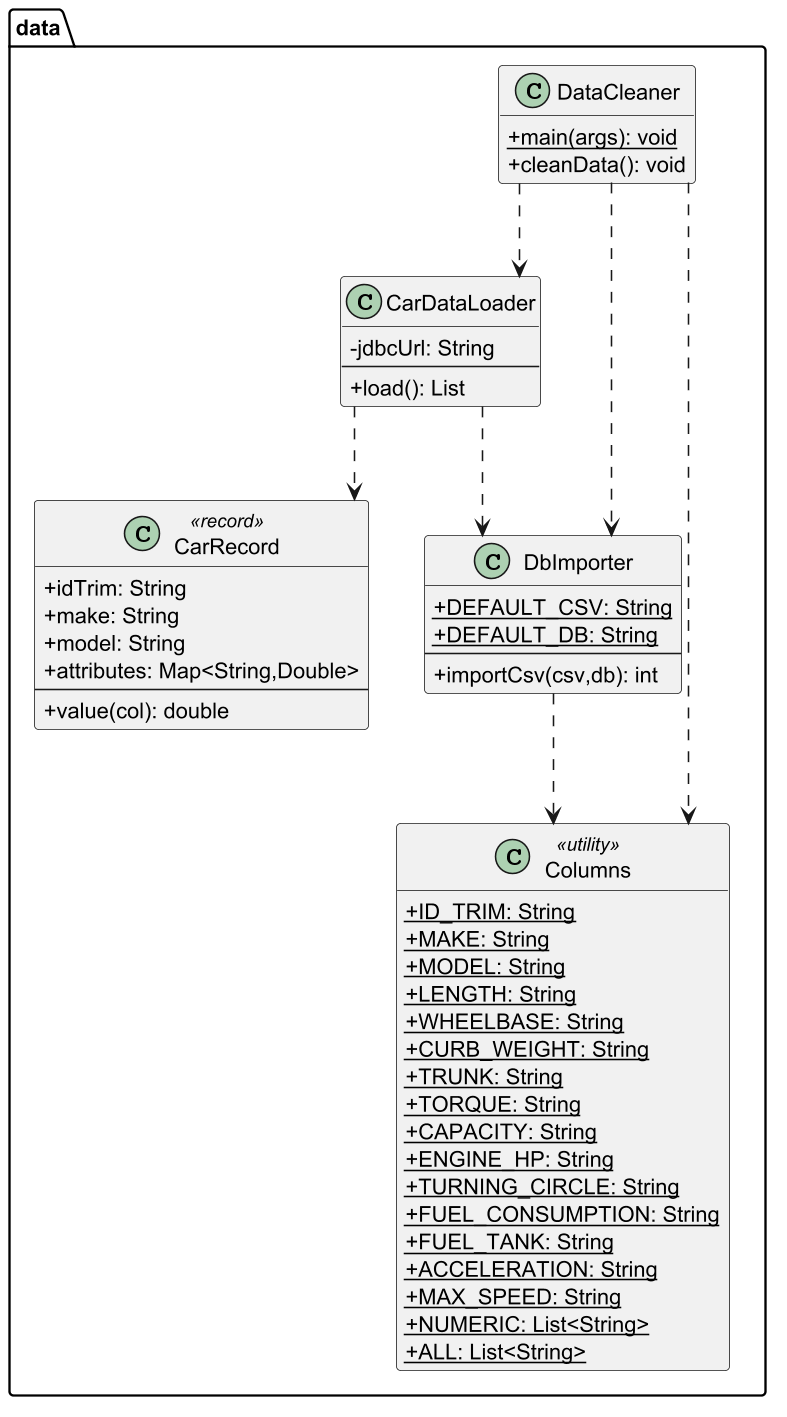
\includegraphics[width=0.78\linewidth]{uml_data.png}
    \caption{Warstwa danych: rekordy, import, czyszczenie i ładowanie.}
\end{figure}

\section{Zbiory klasyczne i zbiory rozmyte}

\subsection{Zbiór klasyczny}

W zbiorze klasycznym obiekt albo należy do zbioru, albo nie należy. Funkcja charakterystyczna ma tylko wartości 0 lub 1:

\[
\chi_A(x) =
\begin{cases}
1, & x \in A\\
0, & x \notin A
\end{cases}
\]

Jeżeli zdefiniujemy klasycznie \emph{samochody szybkie} jako te z prędkością maksymalną co najmniej 200 km/h, to auto z prędkością 199 km/h nie jest szybkie, a auto z prędkością 200 km/h jest szybkie. To jest proste, ale często zbyt brutalne.

\subsection{Zbiór rozmyty}

Zbiór rozmyty \(A\) opisuje funkcja przynależności:

\[
\mu_A : X \rightarrow [0,1]
\]

Wartość \(\mu_A(x)\) oznacza, w jakim stopniu element \(x\) należy do zbioru \(A\):

\begin{itemize}
    \item \(0\): element w ogóle nie należy;
    \item \(1\): element należy w pełni;
    \item wartości między 0 i 1: element należy częściowo.
\end{itemize}

Przykład:

\[
\mu_{\text{szybki}}(190)=0.4,\quad
\mu_{\text{szybki}}(210)=0.8,\quad
\mu_{\text{szybki}}(250)=1.0
\]

Takie podejście jest naturalne, bo wiele pojęć językowych ma granice płynne, nie ostre.

\subsection{Uniwersum}

\term{Uniwersum} to dziedzina wartości, na której działa zbiór rozmyty. Dla prędkości maksymalnej może to być np. przedział od 0 do 400 km/h. W kodzie odpowiada za to klasa \code{Universe}.

W projekcie uniwersum potrafi być:

\begin{itemize}
    \item \term{ciągłe}: np. prędkość, masa, długość;
    \item \term{dyskretne}: gdyby analizowane wartości były skończonym zestawem punktów.
\end{itemize}

Klasa \code{Universe} udostępnia między innymi punkty próbkowania. Są potrzebne, ponieważ wiele własności zbiorów rozmytych, np. nośnik albo kardynalność, jest w projekcie liczona numerycznie przez przejście po próbkach dziedziny.

\subsection{Funkcje przynależności}

Funkcja przynależności mówi, jak wartość liczbowa zamienia się w stopień spełnienia etykiety. W projekcie są zaimplementowane trzy typy funkcji:

\begin{longtable}{p{0.22\linewidth}p{0.34\linewidth}p{0.34\linewidth}}
\toprule
\textbf{Funkcja} & \textbf{Parametry} & \textbf{Intuicja}\\
\midrule
\endhead
trójkątna & \(a,b,c\) & rośnie liniowo do maksimum w \(b\), potem liniowo maleje\\
trapezoidalna & \(a,b,c,d\) & ma lewy stok, plateau z wartością 1 i prawy stok\\
gaussowska & \(c,\sigma\) & gładki dzwon wokół środka \(c\)\\
\bottomrule
\end{longtable}

Kodowo odpowiadają im klasy:

\begin{itemize}
    \item \code{TriangularMf};
    \item \code{TrapezoidalMf};
    \item \code{GaussianMf}.
\end{itemize}

Najczęściej używana jest funkcja trapezoidalna, bo dobrze modeluje etykiety językowe typu \emph{mały}, \emph{średni}, \emph{duży}: istnieje zakres, w którym etykieta pasuje w pełni, oraz zakresy przejściowe.

\begin{figure}[htbp]
    \centering
    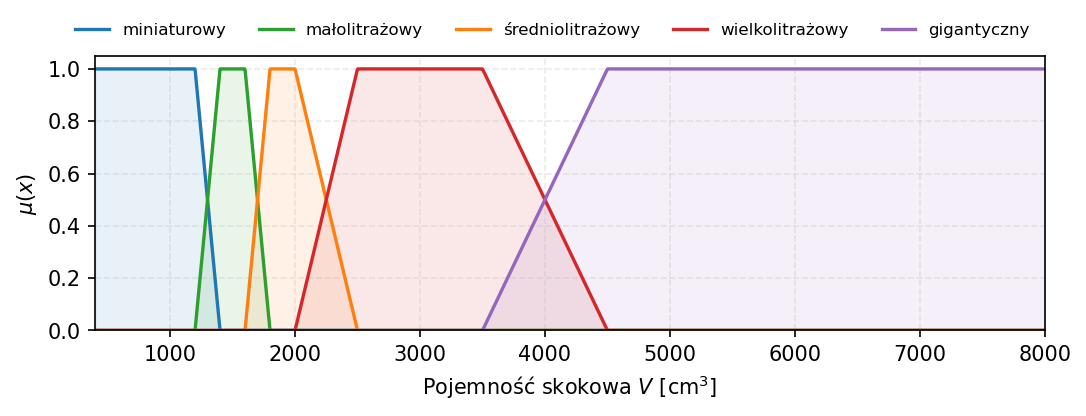
\includegraphics[width=0.82\linewidth]{mf_capacity_cm3.png}
    \caption{Przykładowe etykiety zmiennej lingwistycznej dla pojemności silnika.}
\end{figure}

\subsection{Wysokość, nośnik, alfa-przekrój, normalność}

Dla zbioru rozmytego ważne są pojęcia pomocnicze:

\begin{description}
    \item[Wysokość] największa wartość funkcji przynależności:
    \[
    h(A)=\sup_{x \in X}\mu_A(x)
    \]
    Jeżeli wysokość wynosi 1, zbiór gdzieś osiąga pełną przynależność.

    \item[Nośnik] zbiór wartości, dla których przynależność jest dodatnia:
    \[
    supp(A)=\{x \in X : \mu_A(x)>0\}
    \]

    \item[Alfa-przekrój] zbiór wartości, których przynależność jest co najmniej \(\alpha\):
    \[
    A_\alpha=\{x \in X : \mu_A(x)\ge\alpha\}
    \]

    \item[Normalność] zbiór jest normalny, jeżeli jego wysokość wynosi 1.

    \item[Pustość] zbiór jest pusty, gdy nigdzie nie ma dodatniej przynależności.

    \item[Wypukłość rozmyta] intuicyjnie: przekroje alfa są spójne; dla typowych etykiet trójkątnych i trapezoidalnych jest to spełnione.
\end{description}

Klasa \code{FuzzySet} obsługuje te operacje przez próbkowanie uniwersum.

\subsection{Operacje na zbiorach rozmytych}

W projekcie używane są standardowe operacje Zadeha:

\[
\mu_{\neg A}(x)=1-\mu_A(x)
\]

\[
\mu_{A \cap B}(x)=\min(\mu_A(x), \mu_B(x))
\]

\[
\mu_{A \cup B}(x)=\max(\mu_A(x), \mu_B(x))
\]

To ma bezpośredni związek z językiem:

\begin{itemize}
    \item \emph{mały i lekki} oznacza minimum z dwóch stopni;
    \item \emph{mały lub lekki} oznacza maksimum z dwóch stopni;
    \item \emph{nie mały} oznacza dopełnienie.
\end{itemize}

W kodzie operacje są w \code{FuzzySet} oraz w pomocniczej klasie \code{Operations}. Łączniki zdań są opisane przez enum \code{Connective}: \code{AND} używa minimum, a \code{OR} maksimum.

\section{Zmienne lingwistyczne i etykiety}

\subsection{Zmienna lingwistyczna}

\term{Zmienna lingwistyczna} to atrybut, którego wartości opisujemy słowami. Formalnie można myśleć o niej jako o zestawie:

\[
\langle \text{nazwa}, \text{dziedzina}, \text{etykiety} \rangle
\]

W projekcie przykładem zmiennej lingwistycznej jest:

\begin{center}
\emph{pojemność silnika}
\end{center}

Jej dziedziną są wartości w cm\(^3\), a etykietami mogą być np.:

\begin{itemize}
    \item \emph{bardzo mała pojemność};
    \item \emph{mała pojemność};
    \item \emph{średnia pojemność};
    \item \emph{duża pojemność};
    \item \emph{bardzo duża pojemność}.
\end{itemize}

W kodzie zmienna lingwistyczna to \code{LinguisticVariable}. Przechowuje:

\begin{itemize}
    \item nazwę wyświetlaną użytkownikowi;
    \item nazwę kolumny w rekordzie;
    \item uniwersum;
    \item listę etykiet;
    \item metodę \code{degreeOf}, która liczy stopień przynależności wartości do wybranej etykiety.
\end{itemize}

\subsection{Etykieta lingwistyczna}

\term{Etykieta} to pojedyncze słowne pojęcie na zmiennej lingwistycznej. Na przykład dla zmiennej \emph{moc silnika} etykietą może być \emph{duża moc}. Etykieta ma nazwę i zbiór rozmyty, czyli funkcję przynależności.

W kodzie etykieta to rekord \code{Label}. Jej znaczenie jest krótkie, ale fundamentalne: bez etykiet nie ma sumaryzatorów ani kwalifikatorów.

\subsection{Etykiety skonfigurowane w projekcie}

Każda z 12 zmiennych liczbowych ma po 5 etykiet trapezoidalnych. Dzięki temu aplikacja może tworzyć wiele zdań automatycznie.

\begin{longtable}{p{0.40\linewidth}p{0.50\linewidth}}
\toprule
\textbf{Zmienna} & \textbf{Typowe etykiety}\\
\midrule
\endhead
długość samochodu & bardzo krótki, krótki, średniej długości, długi, bardzo długi\\
rozstaw osi & bardzo mały, mały, średni, duży, bardzo duży\\
masa własna & bardzo lekki, lekki, średniej masy, ciężki, bardzo ciężki\\
pojemność bagażnika & bardzo mała, mała, średnia, duża, bardzo duża\\
moment obrotowy & bardzo mały, mały, średni, duży, bardzo duży\\
pojemność silnika & bardzo mała, mała, średnia, duża, bardzo duża\\
moc silnika & bardzo mała, mała, średnia, duża, bardzo duża\\
średnica zawracania & bardzo mała, mała, średnia, duża, bardzo duża\\
spalanie mieszane & bardzo niskie, niskie, średnie, wysokie, bardzo wysokie\\
pojemność zbiornika paliwa & bardzo mała, mała, średnia, duża, bardzo duża\\
przyspieszenie 0--100 & bardzo szybkie, szybkie, średnie, wolne, bardzo wolne\\
prędkość maksymalna & bardzo mała, mała, średnia, duża, bardzo duża\\
\bottomrule
\end{longtable}

Nazwy etykiet są ważne nie tylko matematycznie, ale też językowo, bo trafiają bezpośrednio do generowanych zdań.

\section{Kwantyfikatory}

\subsection{Czym jest kwantyfikator}

\term{Kwantyfikator} mówi, jak dużej części zbioru dotyczy zdanie. W klasycznej logice mamy kwantyfikatory ostre, np.:

\begin{itemize}
    \item \emph{dla każdego};
    \item \emph{istnieje};
    \item \emph{co najmniej jeden}.
\end{itemize}

W podsumowaniach lingwistycznych używamy kwantyfikatorów rozmytych:

\begin{itemize}
    \item \emph{prawie żaden};
    \item \emph{mniejszość};
    \item \emph{około połowy};
    \item \emph{większość};
    \item \emph{prawie wszystkie};
    \item \emph{kilka tysięcy};
    \item \emph{kilkanaście tysięcy};
    \item \emph{dużo}.
\end{itemize}

Kwantyfikator też jest zbiorem rozmytym, tylko jego dziedziną nie jest np. prędkość samochodu, lecz liczność albo proporcja.

\subsection{Kwantyfikator względny}

Kwantyfikator względny działa na proporcji z przedziału \([0,1]\). Na przykład:

\[
\text{udział samochodów spełniających } S = 0.72
\]

Wtedy pytamy, w jakim stopniu 0.72 pasuje do kwantyfikatora \emph{większość}.

W projekcie skonfigurowano:

\begin{longtable}{p{0.25\linewidth}p{0.45\linewidth}p{0.20\linewidth}}
\toprule
\textbf{Kwantyfikator} & \textbf{Parametry trapezu} & \textbf{Typ}\\
\midrule
\endhead
prawie żaden & \(0,0,0.05,0.20\) & względny\\
mniejszość & \(0.05,0.20,0.30,0.40\) & względny\\
około połowy & \(0.30,0.40,0.60,0.70\) & względny\\
większość & \(0.60,0.70,0.85,0.95\) & względny\\
prawie wszystkie & \(0.85,0.95,1,1\) & względny\\
\bottomrule
\end{longtable}

\begin{figure}[htbp]
    \centering
    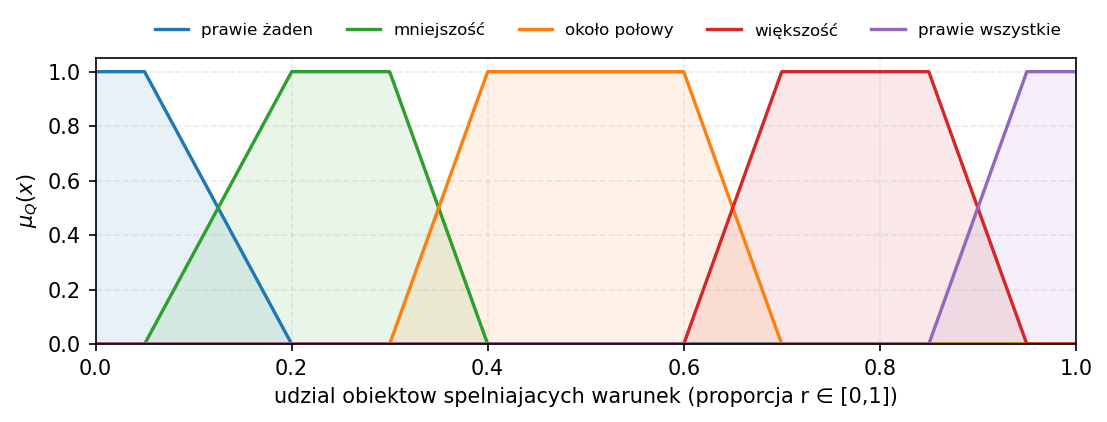
\includegraphics[width=0.82\linewidth]{quantifiers_relative.png}
    \caption{Kwantyfikatory względne używane w projekcie.}
\end{figure}

\subsection{Kwantyfikator absolutny}

Kwantyfikator absolutny działa na liczności, a nie na proporcji. Przykład:

\[
\text{sumaryczna liczba samochodów spełniających } S = 7800
\]

Wtedy sprawdzamy, jak 7800 pasuje do kwantyfikatora \emph{kilka tysięcy} albo \emph{kilkanaście tysięcy}.

W projekcie skonfigurowano:

\begin{longtable}{p{0.25\linewidth}p{0.45\linewidth}p{0.20\linewidth}}
\toprule
\textbf{Kwantyfikator} & \textbf{Parametry trapezu} & \textbf{Typ}\\
\midrule
\endhead
bardzo mało & \(0,0,1000,3000\) & absolutny\\
kilka tysięcy & \(1000,3000,6000,8000\) & absolutny\\
kilkanaście tysięcy & \(6000,8000,14000,16000\) & absolutny\\
dużo & \(14000,16000,25000,25000\) & absolutny\\
\bottomrule
\end{longtable}

\begin{figure}[htbp]
    \centering
    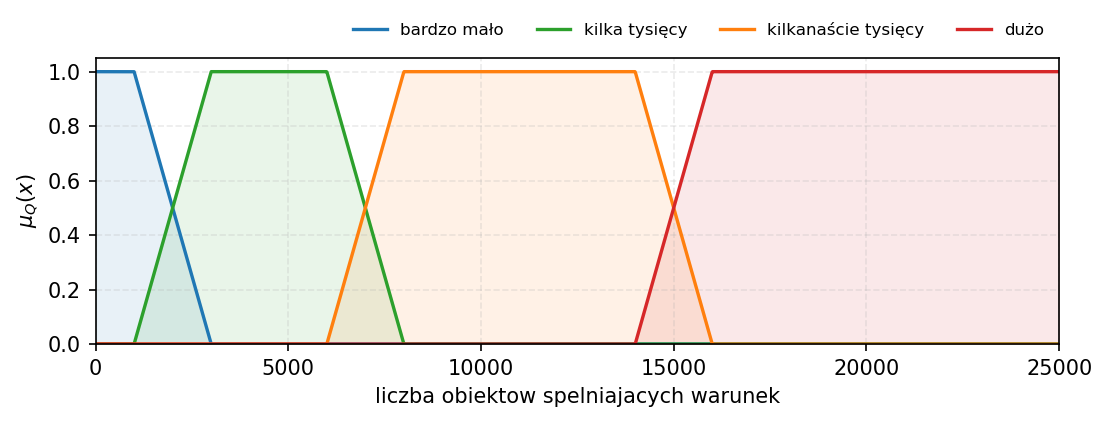
\includegraphics[width=0.82\linewidth]{quantifiers_absolute.png}
    \caption{Kwantyfikatory absolutne używane w projekcie.}
\end{figure}

\subsection{Kwantyfikator w kodzie}

W kodzie kwantyfikator to \code{Quantifier}. Przechowuje nazwę, typ i zbiór rozmyty. Najważniejsza metoda to \code{degree(quantity)}, czyli odpowiedź na pytanie:

\begin{center}
\emph{W jakim stopniu ta proporcja albo ta liczba pasuje do tego kwantyfikatora?}
\end{center}

Jeżeli kwantyfikator jest względny, argument powinien być proporcją. Jeżeli jest absolutny, argument powinien być licznością. Poprawny dobór argumentu jest istotny, bo \emph{większość} nie ma sensu dla liczby 12000, a \emph{kilka tysięcy} nie ma sensu dla wartości 0.6.

\section{Sumaryzator, kwalifikator i podmiot}

\subsection{Sumaryzator}

\term{Sumaryzator} to właściwość, którą przypisujemy obiektom. W zdaniu:

\begin{center}
\emph{Większość samochodów ma dużą moc silnika.}
\end{center}

sumaryzatorem jest:

\begin{center}
\emph{ma dużą moc silnika}
\end{center}

Sumaryzator może być prosty, gdy składa się z jednej etykiety, albo złożony, gdy łączy dwie etykiety spójnikiem:

\begin{itemize}
    \item prosty: \emph{ma dużą moc silnika};
    \item złożony z \emph{i}: \emph{ma dużą moc silnika i niskie spalanie};
    \item złożony z \emph{lub}: \emph{ma dużą moc silnika lub dużą prędkość maksymalną}.
\end{itemize}

Kodowo atomowym sumaryzatorem jest \code{Property}. To obiekt łączący zmienną lingwistyczną z etykietą. \code{Property.degree(record)} pobiera z rekordu odpowiednią kolumnę i liczy stopień przynależności wartości do etykiety.

\subsection{Kwalifikator}

\term{Kwalifikator} zawęża zbiór obiektów, o których mówimy. Zdanie z kwalifikatorem ma postać:

\[
Q\;Y\;\text{będących}\;R\;\text{jest/są}\;S
\]

Przykład:

\begin{center}
\emph{Większość samochodów o dużym bagażniku ma dużą masę własną.}
\end{center}

Tutaj:

\begin{itemize}
    \item \(Q=\) \emph{większość};
    \item \(Y=\) samochody;
    \item \(R=\) \emph{o dużym bagażniku};
    \item \(S=\) \emph{ma dużą masę własną}.
\end{itemize}

Kwalifikator działa jak filtr, ale filtr rozmyty. Samochód może należeć do grupy \emph{o dużym bagażniku} w stopniu 0.2, 0.7 albo 1.0. Dlatego w obliczeniach nie wyrzucamy rekordów zero-jedynkowo, tylko ważymy je stopniem spełnienia kwalifikatora.

\subsection{Podmiot}

W podsumowaniach jednopodmiotowych podmiotem jest cały zbiór samochodów. W podsumowaniach wielopodmiotowych podmiotami są grupy samochodów, np. marki:

\begin{itemize}
    \item samochody marki BMW;
    \item samochody marki Toyota;
    \item samochody marki Ford.
\end{itemize}

Kodowo podmiot wielopodmiotowy to \code{Subject}. Najczęściej powstaje przez \code{Subject.ofMake(make)}, czyli przez predykat wybierający rekordy o konkretnej marce.

\section{Podsumowania jednopodmiotowe}

\subsection{Forma pierwsza}

Forma pierwsza nie ma kwalifikatora:

\[
Q\;Y\;\text{jest/są}\;S
\]

Przykłady:

\begin{itemize}
    \item \emph{Większość samochodów ma małą pojemność silnika.}
    \item \emph{Około połowy samochodów ma średnią prędkość maksymalną.}
    \item \emph{Kilka tysięcy samochodów ma bardzo duży moment obrotowy.}
\end{itemize}

W kodzie forma pierwsza powstaje metodami:

\begin{itemize}
    \item \code{SummaryGenerator.simpleForm1} dla pojedynczego sumaryzatora;
    \item \code{SummaryGenerator.compoundForm1} dla dwóch sumaryzatorów połączonych \code{AND} albo \code{OR}.
\end{itemize}

\subsection{Forma druga}

Forma druga ma kwalifikator:

\[
Q\;Y\;\text{będących}\;R\;\text{jest/są}\;S
\]

Przykłady:

\begin{itemize}
    \item \emph{Większość samochodów o dużej mocy silnika ma dużą prędkość maksymalną.}
    \item \emph{Mniejszość samochodów o niskim spalaniu ma bardzo dużą masę własną.}
    \item \emph{Około połowy samochodów z dużym bagażnikiem ma duży rozstaw osi.}
\end{itemize}

W kodzie forma druga powstaje metodą:

\begin{itemize}
    \item \code{SummaryGenerator.simpleForm2}.
\end{itemize}

Projekt pilnuje, żeby kwalifikator i sumaryzator nie były tą samą prostą właściwością. Zdanie typu \emph{Większość samochodów będących szybkimi jest szybka} byłoby mało informacyjne.

\subsection{Spójniki AND i OR}

Dla złożonych sumaryzatorów projekt używa:

\[
\mu_{S_1 \land S_2}(y)=\min(\mu_{S_1}(y), \mu_{S_2}(y))
\]

\[
\mu_{S_1 \lor S_2}(y)=\max(\mu_{S_1}(y), \mu_{S_2}(y))
\]

Czyli:

\begin{itemize}
    \item \emph{szybki i ekonomiczny} jest tak mocne, jak słabsza z dwóch cech;
    \item \emph{szybki lub ekonomiczny} jest tak mocne, jak mocniejsza z dwóch cech.
\end{itemize}

To jest jeden z najważniejszych miejsc, w których matematyka zbiorów rozmytych bezpośrednio przekłada się na język.

\subsection{Obiekt podsumowania w kodzie}

Wynikiem generatora jest \code{SingleSubjectSummary}. Ten obiekt przechowuje:

\begin{itemize}
    \item formę: I albo II;
    \item kwantyfikator;
    \item sumaryzator;
    \item opcjonalny kwalifikator;
    \item tekst zdania;
    \item typ kwantyfikatora: względny albo absolutny.
\end{itemize}

Miary jakości nie są częścią samego zdania. Są liczone osobno przez \code{QualityMeasures.evaluate}.

\begin{figure}[htbp]
    \centering
    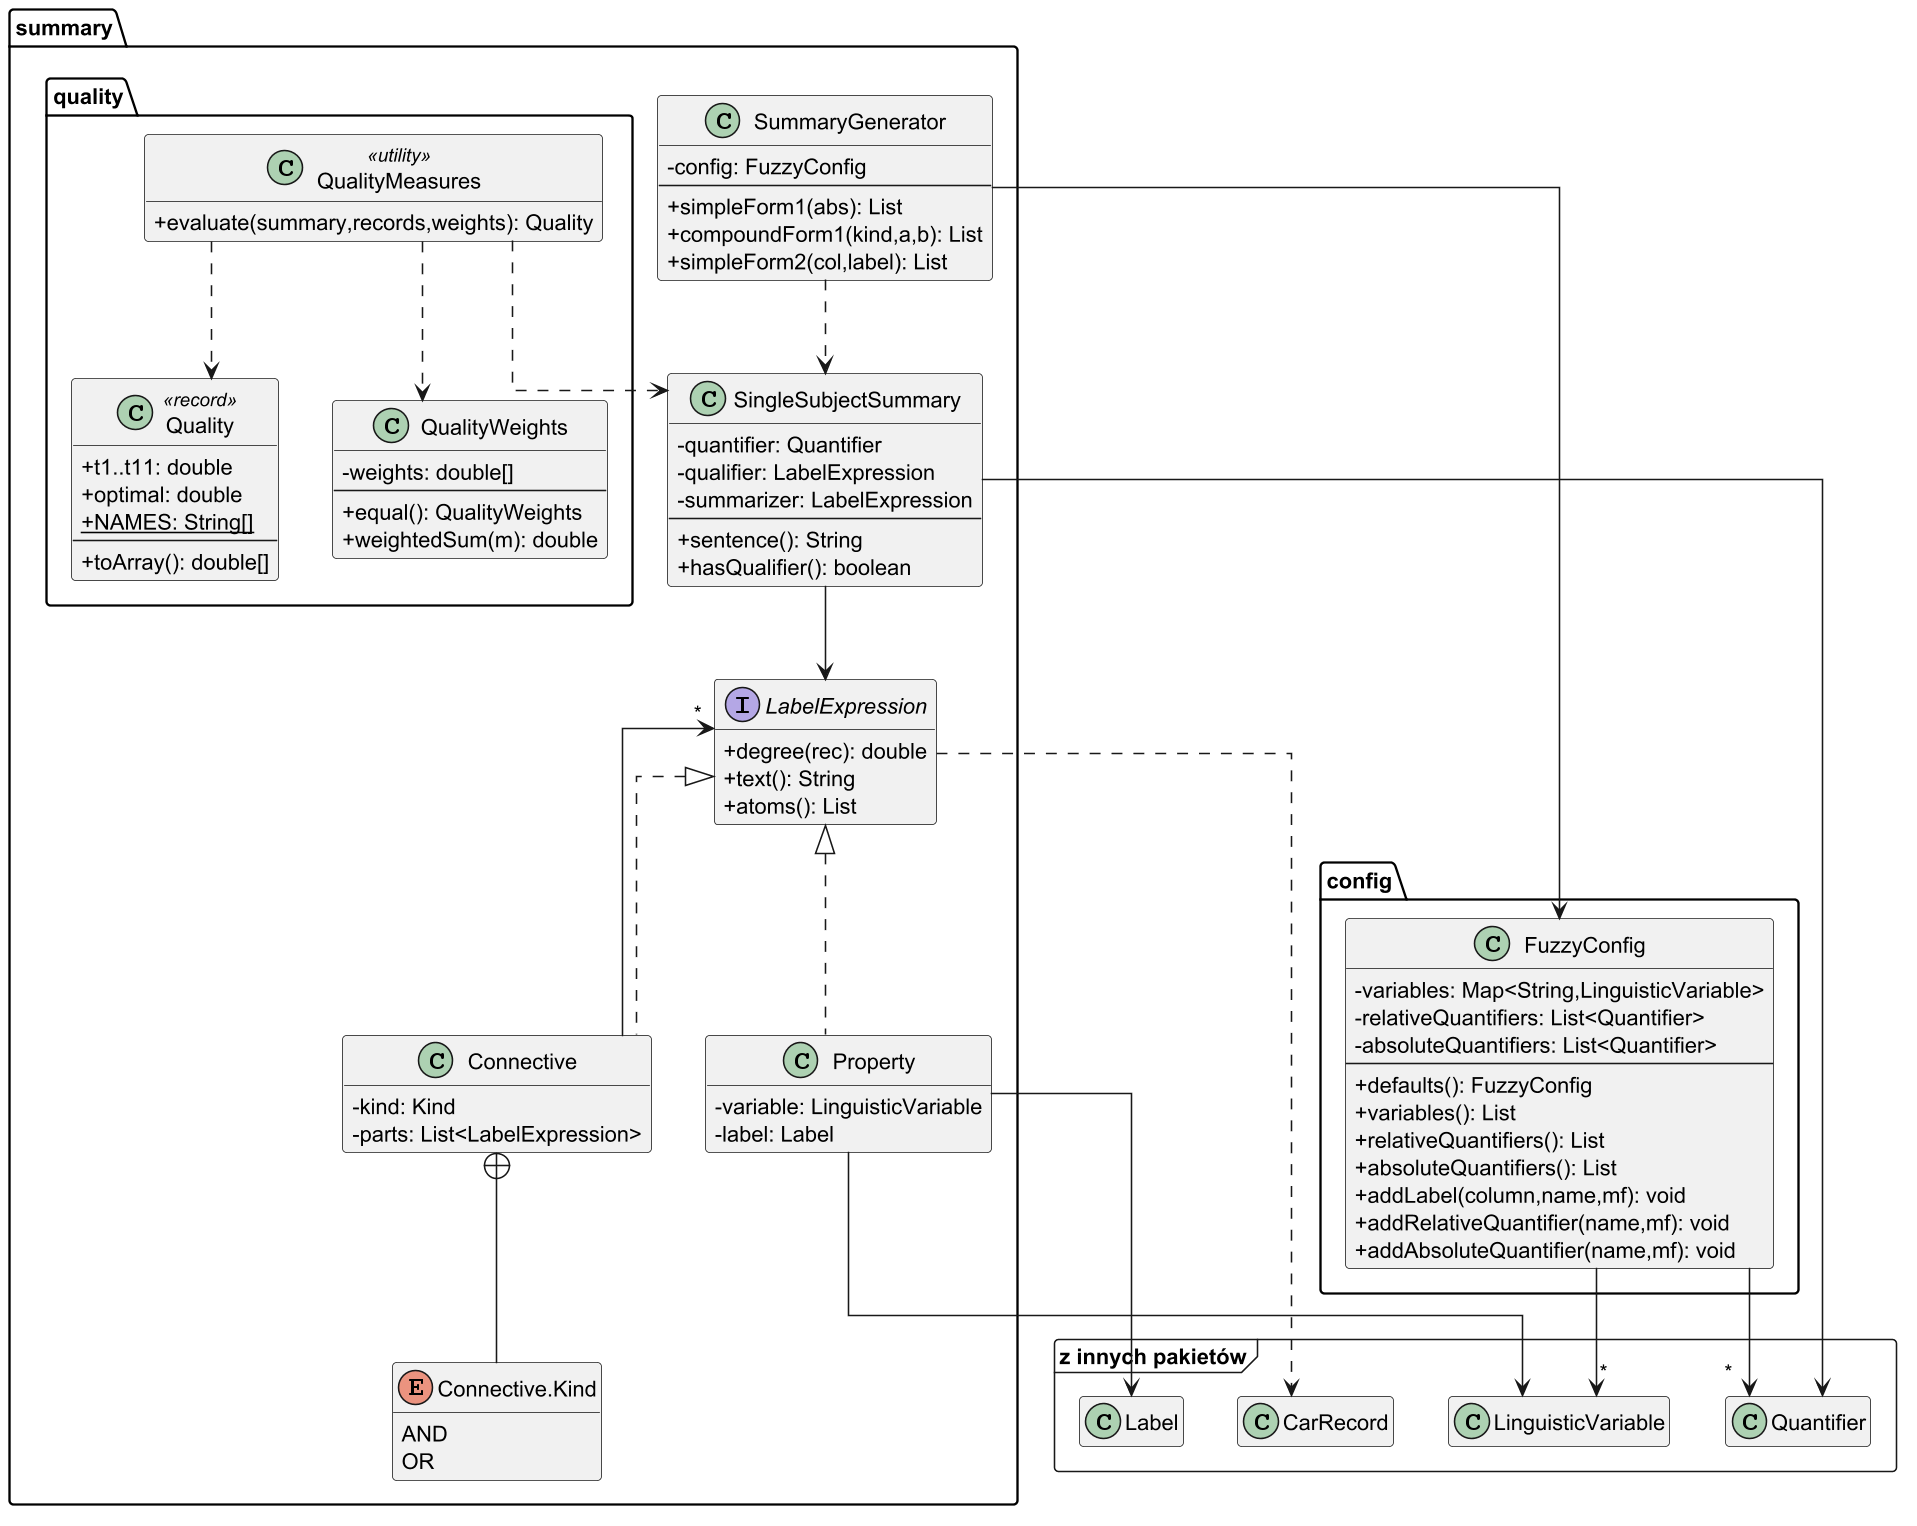
\includegraphics[width=0.94\linewidth]{uml_summary.png}
    \caption{Kluczowe klasy dla podsumowań jednopodmiotowych.}
\end{figure}

\section{Stopień prawdziwości T1}

\subsection{Dlaczego T1 jest najważniejsze}

Miara T1 to \term{stopień prawdziwości podsumowania}. Odpowiada na pytanie:

\begin{center}
\emph{Na ile dane rzeczywiście potwierdzają wygenerowane zdanie?}
\end{center}

To jest najbliższy odpowiednik prawdy logicznej, ale w przedziale \([0,1]\).

\subsection{Forma I z kwantyfikatorem względnym}

Dla zdania:

\[
Q\;Y\;\text{jest/są}\;S
\]

liczymy średni stopień spełnienia sumaryzatora wśród obiektów:

\[
r = \frac{1}{n}\sum_{i=1}^{n}\mu_S(y_i)
\]

Następnie sprawdzamy, jak ta proporcja pasuje do kwantyfikatora:

\[
T_1 = \mu_Q(r)
\]

Przykład intuicyjny: jeżeli średni stopień spełnienia etykiety \emph{mała pojemność silnika} wynosi 0.72, to dla kwantyfikatora \emph{większość} wynik może być wysoki.

\subsection{Forma I z kwantyfikatorem absolutnym}

Dla kwantyfikatora absolutnego nie dzielimy przez liczbę rekordów. Liczymy rozmytą liczność:

\[
c = \sum_{i=1}^{n}\mu_S(y_i)
\]

a potem:

\[
T_1 = \mu_Q(c)
\]

Przykład: jeżeli suma przynależności do \emph{dużej mocy} wynosi 7500, to sprawdzamy, czy 7500 pasuje do \emph{kilku tysięcy} albo \emph{kilkunastu tysięcy}.

\subsection{Forma II z kwalifikatorem}

Dla formy:

\[
Q\;Y\;\text{będących}\;R\;\text{jest/są}\;S
\]

kwalifikator ogranicza zbiór obiektów. W wersji względnej liczymy:

\[
r = \frac{\sum_{i=1}^{n}\min(\mu_R(y_i), \mu_S(y_i))}
{\sum_{i=1}^{n}\mu_R(y_i)}
\]

i następnie:

\[
T_1 = \mu_Q(r)
\]

W liczniku jest część kwalifikowanych obiektów, która spełnia też sumaryzator. W mianowniku jest rozmyta liczność obiektów kwalifikowanych.

Jeżeli mianownik wynosi 0, to znaczy, że kwalifikator nie opisuje żadnego obiektu w danych. Projekt zwraca wtedy 0, bo nie ma podstaw do uznania zdania za prawdziwe.

\section{Miary jakości T1--T11}

\subsection{Po co tyle miar}

Samo T1 nie wystarcza. Zdanie może być prawdziwe, ale mało przydatne. Na przykład:

\begin{center}
\emph{Prawie wszystkie samochody mają jakąś długość.}
\end{center}

Mogłoby być bardzo prawdziwe, ale informacyjnie słabe. Dlatego system Yagera/Kacprzyka używa dodatkowych miar: część ocenia prawdziwość, część specyficzność, część prostotę, część informacyjność kwantyfikatora i kwalifikatora.

W projekcie klasa \code{QualityMeasures} liczy 11 miar i wynik optymalny:

\[
OPT = \sum_{i=1}^{11} w_i T_i
\]

gdzie \(w_i\) to waga miary \(T_i\). Wagi są walidowane i normalizowane przez \code{QualityWeights}.

\subsection{Tabela miar}

\begin{longtable}{p{0.08\linewidth}p{0.25\linewidth}p{0.55\linewidth}}
\toprule
\textbf{Miara} & \textbf{Nazwa intuicyjna} & \textbf{Co mierzy}\\
\midrule
\endhead
T1 & prawdziwość & zgodność zdania z danymi po zastosowaniu kwantyfikatora\\
T2 & nieprecyzyjność sumaryzatora & im szersze etykiety sumaryzatora, tym mniejsza wartość tej miary\\
T3 & stopień pokrycia & jaki odsetek obiektów dodatnio spełnia sumaryzator\\
T4 & stopień trafności & różnica między pokryciem rzeczywistym a oczekiwanym przy niezależności atomów\\
T5 & długość podsumowania & premiuje krótsze, prostsze sumaryzatory\\
T6 & nieprecyzyjność kwantyfikatora & premiuje bardziej konkretne kwantyfikatory\\
T7 & kardynalność kwantyfikatora & premiuje kwantyfikatory o mniejszej rozmytej liczności\\
T8 & kardynalność sumaryzatora & premiuje bardziej selektywne sumaryzatory\\
T9 & nieprecyzyjność kwalifikatora & analog T2 dla kwalifikatora, tylko w formie II\\
T10 & kardynalność kwalifikatora & analog T8 dla kwalifikatora, tylko w formie II\\
T11 & długość kwalifikatora & premiuje krótsze kwalifikatory, tylko w formie II\\
\bottomrule
\end{longtable}

\subsection{T1: prawdziwość}

T1 opisano szczegółowo w poprzednim rozdziale. To miara najłatwiejsza do intuicyjnej interpretacji: mówi, czy zdanie pasuje do danych.

W kodzie T1 zależy od:

\begin{itemize}
    \item formy podsumowania;
    \item typu kwantyfikatora;
    \item sumy stopni przynależności do sumaryzatora;
    \item w formie II także od sumy stopni kwalifikatora.
\end{itemize}

\subsection{T2: nieprecyzyjność sumaryzatora}

T2 ocenia, jak szeroki jest sumaryzator. Jeśli etykieta obejmuje bardzo dużą część uniwersum, to jest mało precyzyjna. Jeżeli obejmuje niewielki obszar, jest bardziej konkretna.

W projekcie używana jest względna kardynalność nośnika etykiety:

\[
T_2 = 1 - \sqrt[m]{\prod_{j=1}^{m} suppRel(S_j)}
\]

gdzie \(m\) to liczba atomowych właściwości w sumaryzatorze.

Interpretacja:

\begin{itemize}
    \item wysoka T2: sumaryzator jest precyzyjny;
    \item niska T2: sumaryzator jest szeroki i ogólny.
\end{itemize}

\subsection{T3: stopień pokrycia}

T3 sprawdza, ile obiektów jest dodatnio objętych przez sumaryzator.

Dla formy I:

\[
T_3 = \frac{|\{y_i : \mu_S(y_i)>0\}|}{n}
\]

Dla formy II:

\[
T_3 = \frac{|\{y_i : \mu_R(y_i)>0 \land \mu_S(y_i)>0\}|}
{|\{y_i : \mu_R(y_i)>0\}|}
\]

T3 używa dodatniej przynależności, więc nie patrzy na to, czy stopień wynosi 0.1 czy 0.9. Patrzy tylko, czy obiekt w ogóle został objęty.

\subsection{T4: stopień trafności}

T4 porównuje rzeczywiste pokrycie sumaryzatora z pokryciem oczekiwanym na podstawie pojedynczych atomów. Dla złożonych sumaryzatorów pozwala ocenić, czy kombinacja cech daje coś więcej niż przypadkowe nałożenie szerokich etykiet.

W kodzie:

\[
T_4 = \left|\prod_{j=1}^{m} p_j - T_3\right|
\]

gdzie \(p_j\) to udział rekordów dodatnio spełniających atom \(S_j\).

\subsection{T5: długość podsumowania}

T5 premiuje krótkie podsumowania. W projekcie:

\[
T_5 = 2 \cdot \left(\frac{1}{2}\right)^m
\]

Dla jednego atomu:

\[
T_5 = 1
\]

Dla dwóch atomów:

\[
T_5 = 0.5
\]

To znaczy, że proste zdanie z jednym sumaryzatorem dostaje maksymalną premię za długość, a zdanie złożone jest karane, bo jest mniej zwięzłe.

\subsection{T6 i T7: jakość kwantyfikatora}

T6 i T7 dotyczą kwantyfikatora.

T6 mierzy nieprecyzyjność przez nośnik:

\[
T_6 = 1 - suppRel(Q)
\]

T7 mierzy rozmytą kardynalność:

\[
T_7 = 1 - sigmaRel(Q)
\]

Im kwantyfikator węższy i bardziej konkretny, tym wyższe te miary. \emph{Około połowy} może być dość informacyjne, bo wskazuje środek skali. Bardzo szeroki kwantyfikator byłby mniej użyteczny.

\subsection{T8: kardynalność sumaryzatora}

T8 jest podobna do T2, ale używa rozmytej kardynalności, czyli sumy stopni przynależności, a nie tylko szerokości nośnika:

\[
T_8 = 1 - \sqrt[m]{\prod_{j=1}^{m} sigmaRel(S_j)}
\]

Wysoka T8 oznacza, że sumaryzator jest selektywny w sensie rozmytym.

\subsection{T9--T11: kwalifikator}

T9, T10 i T11 pojawiają się tylko dla formy II. Jeżeli podsumowanie nie ma kwalifikatora, projekt ustawia je na 0.

\begin{itemize}
    \item T9: nieprecyzyjność kwalifikatora;
    \item T10: rozmyta kardynalność kwalifikatora;
    \item T11: długość kwalifikatora.
\end{itemize}

Ich sens jest analogiczny do T2, T8 i T5, tylko dotyczą warunku zawężającego zbiór obiektów.

\subsection{Wynik optymalny}

Wynik optymalny to średnia ważona:

\[
OPT = w_1T_1 + w_2T_2 + \ldots + w_{11}T_{11}
\]

Domyślne wagi mogą sprawić, że zdanie o niezbyt wysokim T1 nadal będzie wysoko w rankingu, jeżeli ma dobry kwantyfikator, precyzyjny sumaryzator i odpowiednią długość. Dlatego podczas interpretacji wyników trzeba zawsze patrzeć na:

\begin{itemize}
    \item T1, gdy interesuje nas prawdziwość;
    \item OPT, gdy interesuje nas kompromis jakości;
    \item T2/T8, gdy chcemy wiedzieć, czy sumaryzator jest konkretny;
    \item T3, gdy chcemy rozumieć pokrycie danych;
    \item T9--T11, gdy analizujemy zdania z kwalifikatorem.
\end{itemize}

\section{Kardynalność i liczność rozmyta}

\subsection{Dlaczego nie liczymy tylko rekordów}

W klasycznym świecie liczność zbioru to liczba elementów. W świecie rozmytym rekord może należeć do zbioru częściowo. Jeśli mamy trzy samochody o stopniach przynależności do etykiety \emph{szybki}:

\[
0.2,\quad 0.8,\quad 1.0
\]

to rozmyta liczność wynosi:

\[
0.2+0.8+1.0=2.0
\]

To znaczy: te trzy rekordy razem dają odpowiednik dwóch pełnych samochodów szybkich.

\subsection{Sigma-count}

W projekcie \term{sigma-count} to suma stopni przynależności po punktach próbkowania albo po rekordach, zależnie od kontekstu.

Dla zbioru rozmytego na uniwersum:

\[
|A|_\Sigma = \sum_{x \in samples(X)} \mu_A(x)
\]

Dla rekordów:

\[
\sum_{i=1}^{n}\mu_S(y_i)
\]

Ta druga suma jest podstawą prawdziwości zdań.

\subsection{Względna kardynalność}

Względna kardynalność dzieli liczność przez rozmiar dziedziny lub liczbę próbek:

\[
sigmaRel(A)=\frac{|A|_\Sigma}{|X|}
\]

Dzięki temu wynik mieści się w \([0,1]\), więc można porównywać etykiety z różnych zmiennych.

\section{Podsumowania wielopodmiotowe}

\subsection{Po co więcej niż jeden podmiot}

Podsumowania jednopodmiotowe mówią o całym zbiorze samochodów. Podsumowania wielopodmiotowe porównują dwie grupy, np. dwie marki. Zamiast pytać:

\begin{center}
\emph{Czy samochody mają dużą moc?}
\end{center}

pytamy:

\begin{center}
\emph{Czy samochody marki BMW częściej niż samochody marki Toyota mają dużą moc?}
\end{center}

To jest inny typ wiedzy: nie opis ogólny, lecz porównanie.

\subsection{Podmioty P1 i P2}

W kodzie podmiot to \code{Subject}. Każdy podmiot ma:

\begin{itemize}
    \item nazwę do zdania;
    \item predykat klasyczny sprawdzający, czy rekord należy do grupy.
\end{itemize}

Dla marek:

\begin{lstlisting}[style=javacode]
Subject p1 = Subject.ofMake("BMW");
Subject p2 = Subject.ofMake("Toyota");
\end{lstlisting}

Projekt pilnuje, żeby P1 i P2 nie były tym samym podmiotem. Porównywanie BMW z BMW nie ma sensu, więc generator odrzuca takie zdania.

\subsection{Cztery formy wielopodmiotowe}

Projekt implementuje formy I--IV.

\begin{longtable}{p{0.12\linewidth}p{0.42\linewidth}p{0.36\linewidth}}
\toprule
\textbf{Forma} & \textbf{Schemat} & \textbf{Intuicja}\\
\midrule
\endhead
I & \(\begin{aligned}[t] QP_1 &\text{ w porównaniu do } P_2\\[-1mm] &\text{ jest } S \end{aligned}\) & porównanie udziału cechy \(S\) w P1 i P2\\
II & \(\begin{aligned}[t] QP_1 \text{ będących } R &\text{ w porównaniu do } P_2\\[-1mm] \text{ będących } R &\text{ jest } S \end{aligned}\) & porównanie obu grup po tym samym zawężeniu\\
III & \(\begin{aligned}[t] QP_1 \text{ będących } R &\text{ w porównaniu do } P_2\\[-1mm] &\text{ jest } S \end{aligned}\) & kwalifikator dotyczy tylko P1\\
IV & \(\begin{aligned}[t] QP_1 &\text{ w porównaniu do } P_2\\[-1mm] &\text{ jest } S \end{aligned}\) & wariant liczony bez normalizacji po liczności grup\\
\bottomrule
\end{longtable}

\subsection{Stopień prawdziwości wielopodmiotowej}

Dla form I--III projekt liczy najpierw siłę sumaryzatora w każdej grupie. W uproszczeniu:

\[
n_1 = \frac{\sum_{y_i \in P_1} \mu_S(y_i)}{|P_1|}
\]

\[
n_2 = \frac{\sum_{y_i \in P_2} \mu_S(y_i)}{|P_2|}
\]

Potem argument kwantyfikatora to:

\[
arg = \frac{n_1}{n_1+n_2}
\]

Jeśli \(arg\) jest blisko 1, cecha silnie dominuje w P1. Jeśli jest blisko 0.5, grupy są podobne. Jeśli jest blisko 0, cecha bardziej pasuje do P2.

Dla formy IV projekt używa:

\[
arg = \frac{\sum_{y_i \in P_1}\mu_S(y_i)}
{\sum_{y_i \in P_1}\mu_S(y_i)+\sum_{y_i \in P_2}\mu_S(y_i)}
\]

Forma IV jest bardziej wrażliwa na liczność grup, bo nie dzieli przez rozmiar podmiotów.

\subsection{Kwalifikator w formach II i III}

W formie II kwalifikator zawęża obie grupy:

\[
P_1 \cap R,\quad P_2 \cap R
\]

W formie III kwalifikator zawęża tylko P1:

\[
P_1 \cap R,\quad P_2
\]

To subtelna, ale ważna różnica. Forma II pyta: ,,wśród podobnie zawężonych obiektów, która grupa ma cechę bardziej?''. Forma III pyta: ,,czy zawężona część P1 wypada wobec całego P2 w określony sposób?''.

\begin{figure}[htbp]
    \centering
    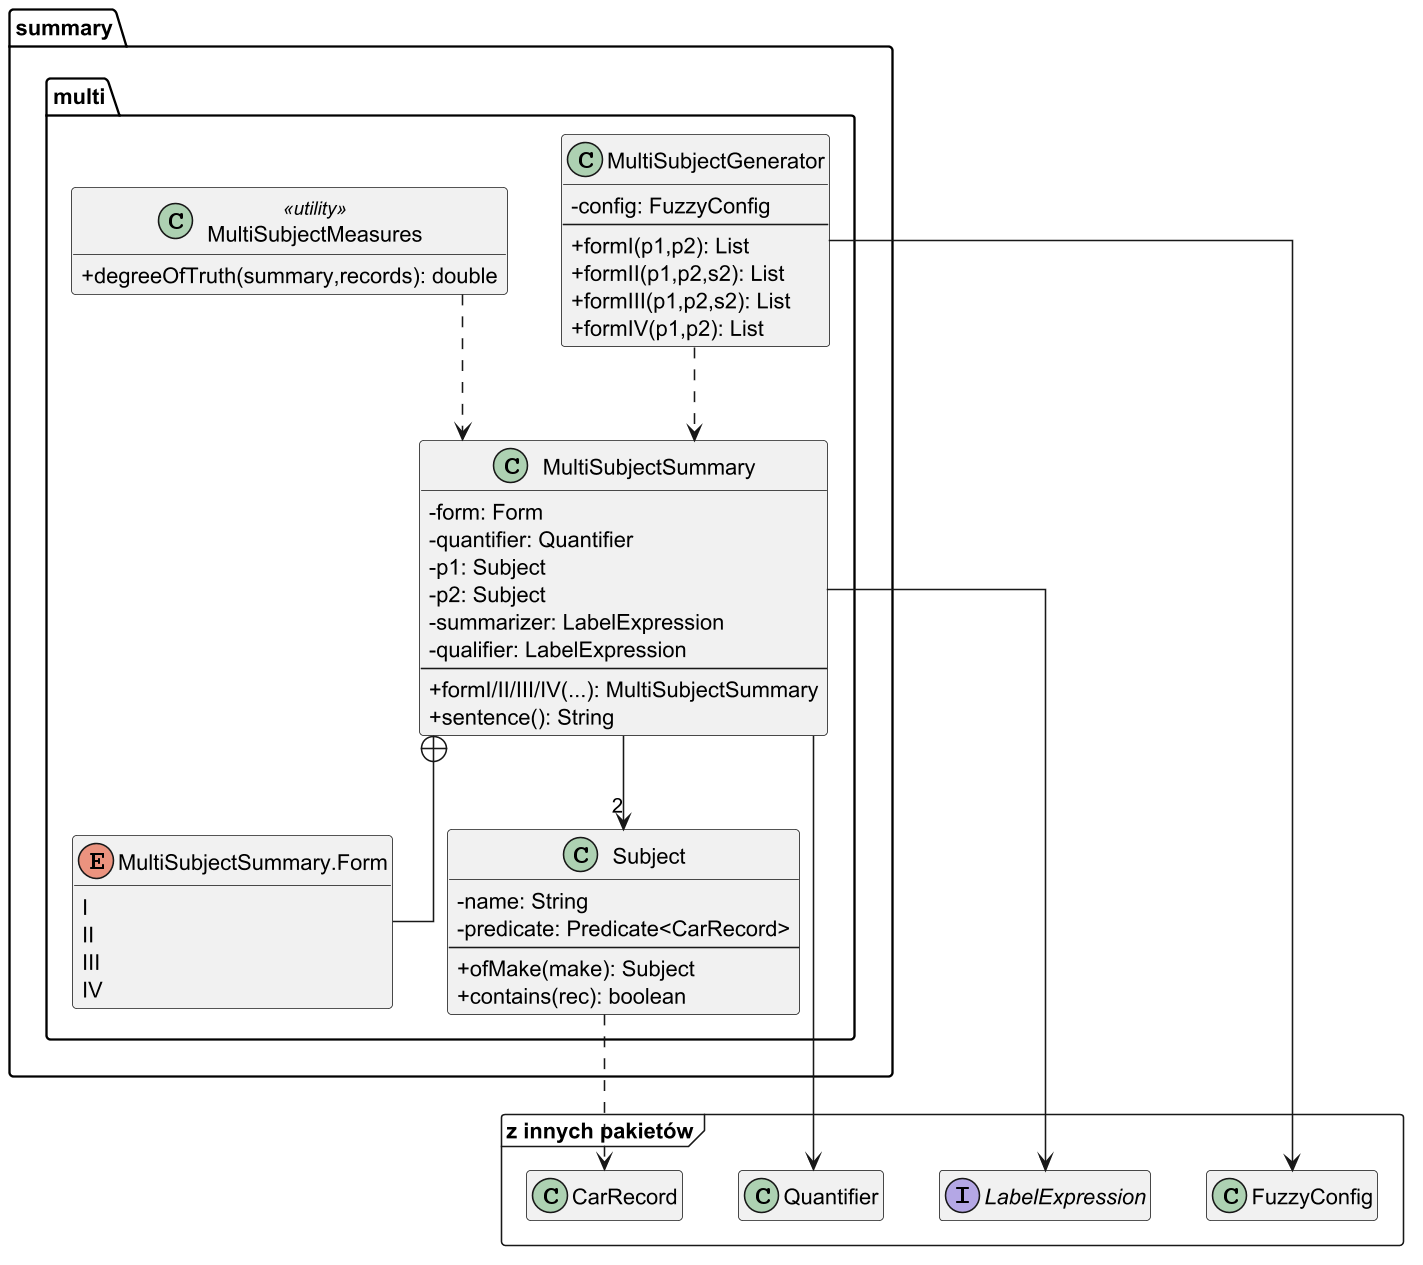
\includegraphics[width=0.94\linewidth]{uml_multi.png}
    \caption{Klasy odpowiedzialne za podsumowania wielopodmiotowe.}
\end{figure}

\section{Architektura kodu}

\subsection{Pakiety}

Kod jest podzielony na kilka pakietów:

\begin{longtable}{p{0.32\linewidth}p{0.58\linewidth}}
\toprule
\textbf{Pakiet} & \textbf{Odpowiedzialność}\\
\midrule
\endhead
\code{org.kosowskinowak.app} & punkt startowy aplikacji\\
\code{org.kosowskinowak.app.gui} & interfejs Swing\\
\code{org.kosowskinowak.config} & konfiguracja zmiennych, etykiet i kwantyfikatorów\\
\code{org.kosowskinowak.data} & rekordy, kolumny, import, czyszczenie i ładowanie danych\\
\code{org.kosowskinowak.fuzzy.mf} & funkcje przynależności\\
\smallcode{org.kosowskinowak.fuzzy.set} & zbiory klasyczne, zbiory rozmyte, uniwersa\\
\smallcode{org.kosowskinowak.fuzzy.linguistic} & zmienne lingwistyczne, etykiety, kwantyfikatory\\
\code{org.kosowskinowak.summary} & podsumowania jednopodmiotowe\\
\smallcode{org.kosowskinowak.summary.quality} & miary T1--T11 i wagi\\
\smallcode{org.kosowskinowak.summary.multi} & podsumowania wielopodmiotowe\\
\bottomrule
\end{longtable}

\begin{figure}[htbp]
    \centering
    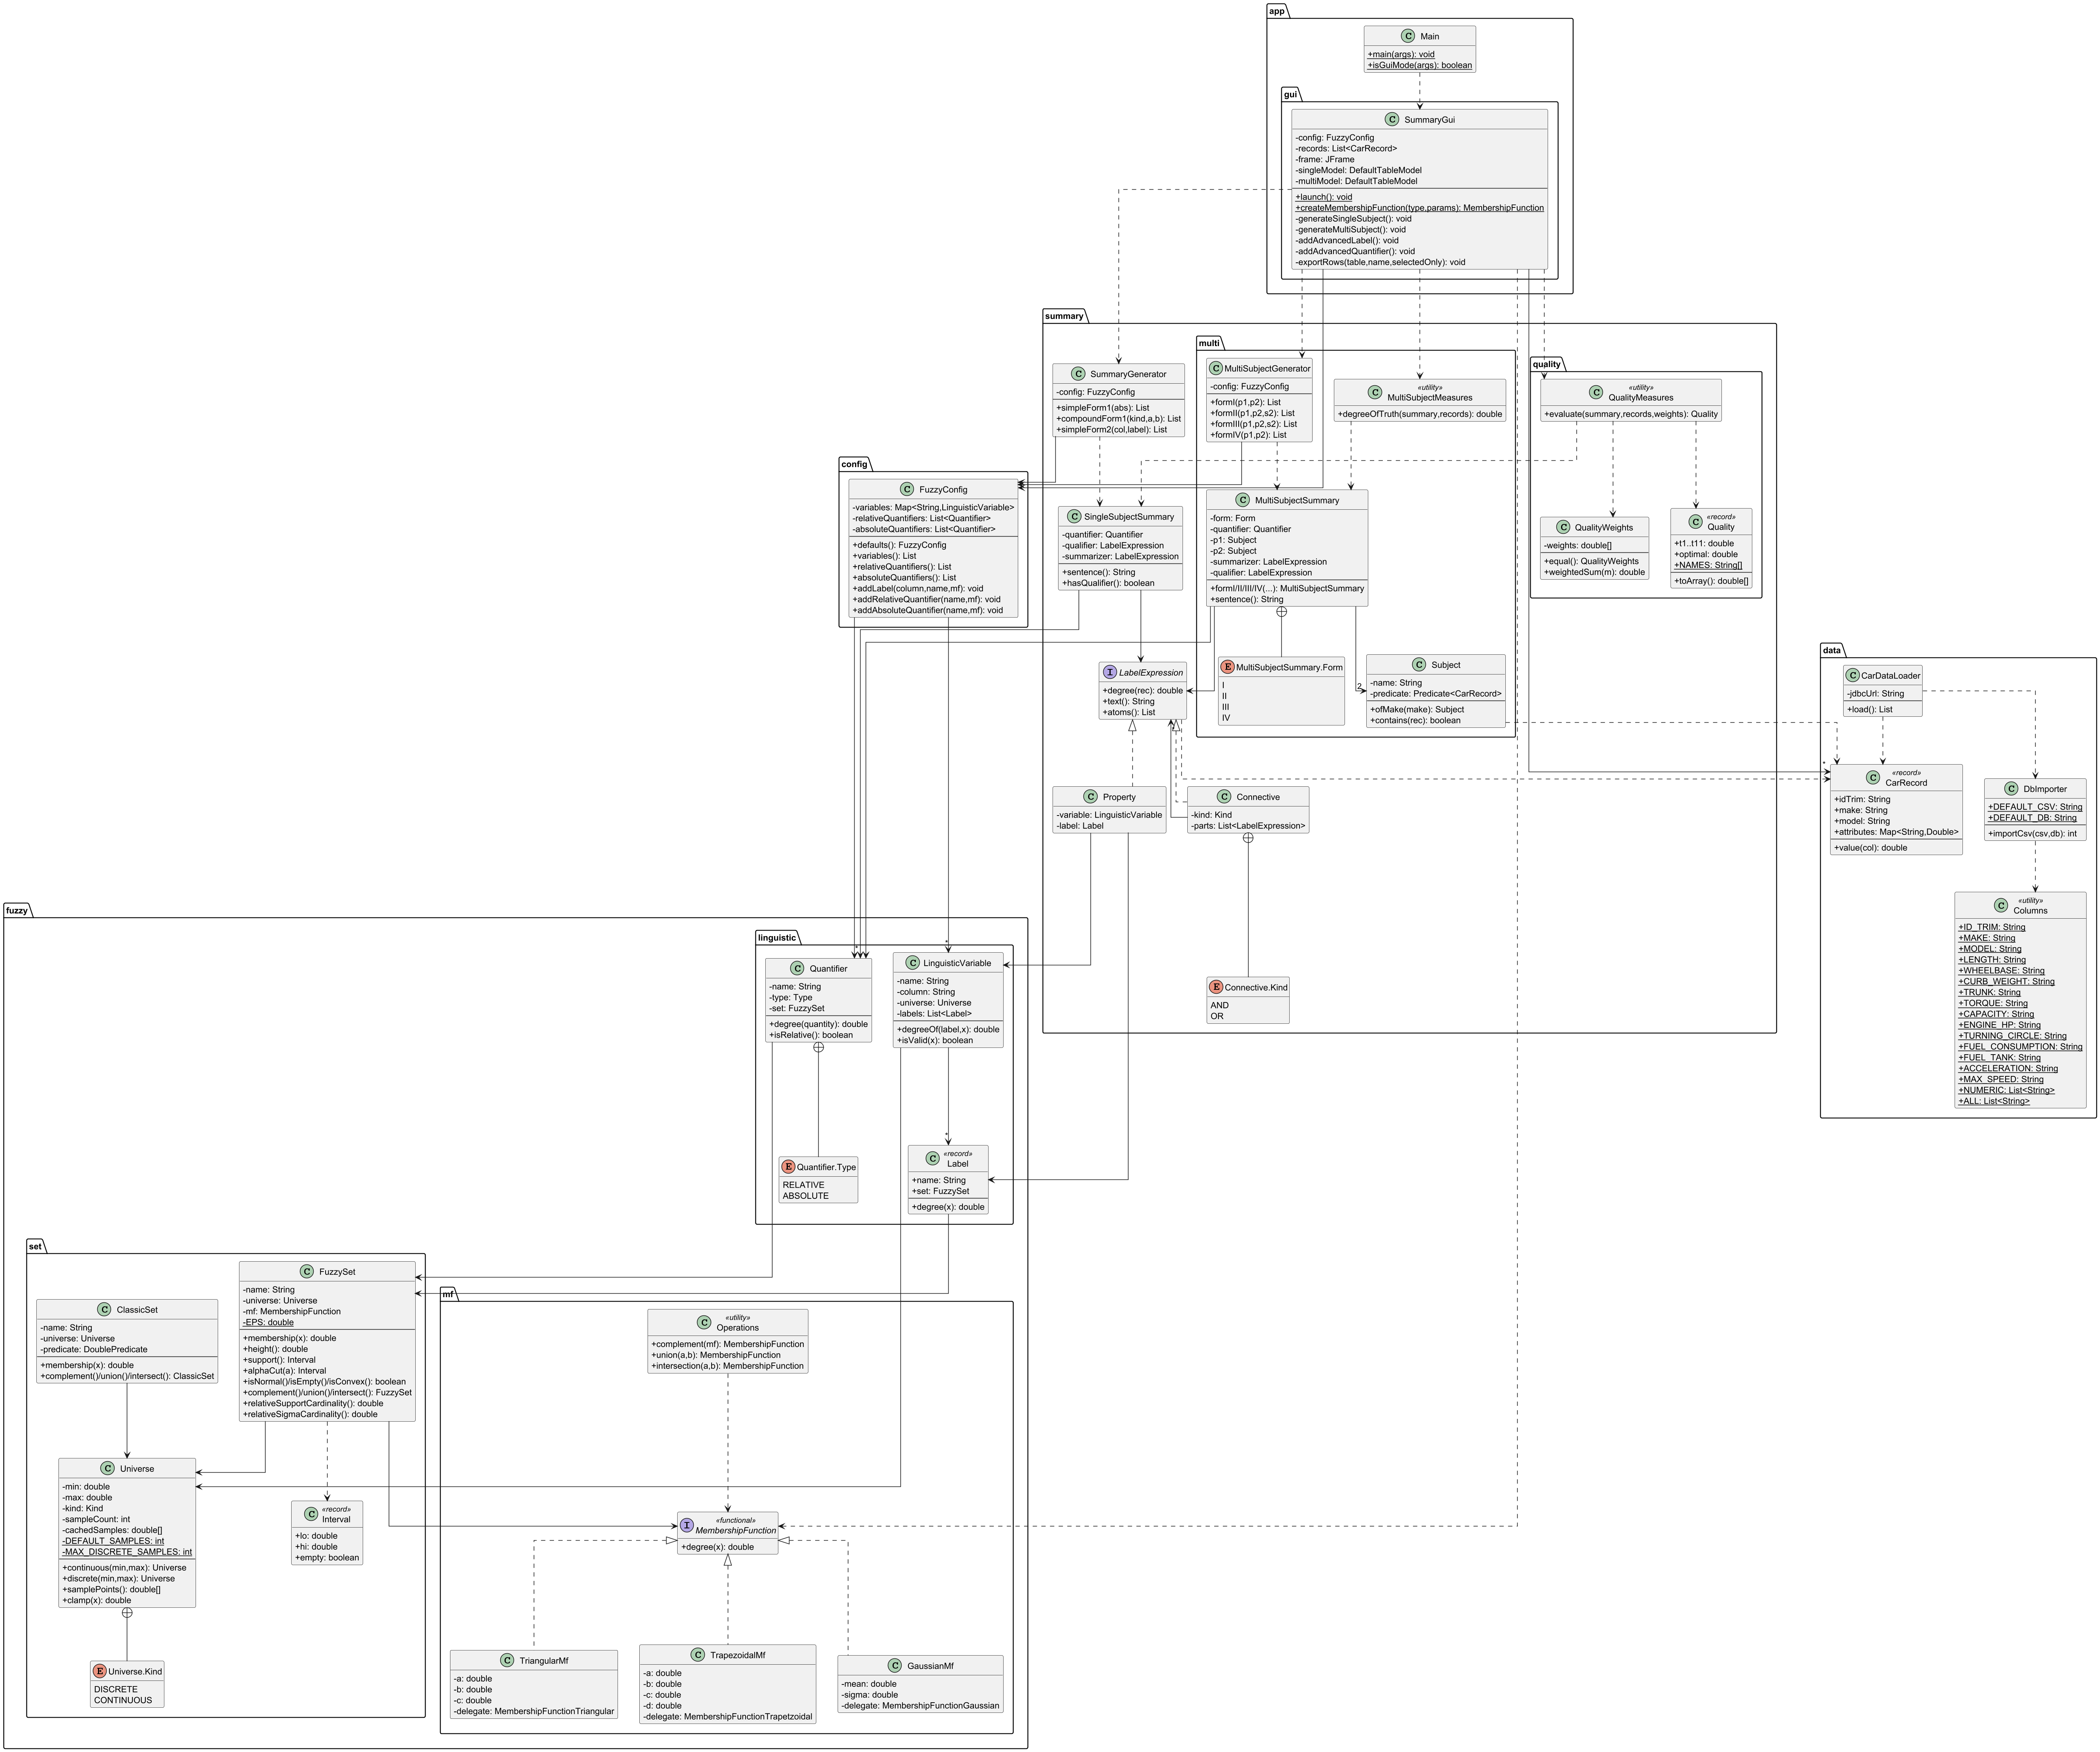
\includegraphics[width=0.88\linewidth]{uml_classes.png}
    \caption{Ogólny diagram klas projektu.}
\end{figure}

\subsection{Warstwa funkcji przynależności}

Interfejs \code{MembershipFunction} definiuje jedną rzecz: dla wartości liczbowej zwrócić stopień przynależności. Dzięki temu reszta systemu nie musi wiedzieć, czy funkcja jest trójkątna, trapezoidalna czy gaussowska.

W przybliżeniu:

\begin{lstlisting}[style=javacode]
public interface MembershipFunction {
    double value(double x);
}
\end{lstlisting}

To prosta abstrakcja, ale bardzo ważna. Pozwala w trybie zaawansowanym GUI dodawać nowe etykiety z różnymi kształtami funkcji.

\subsection{Warstwa zbiorów}

\code{FuzzySet} łączy funkcję przynależności z uniwersum. Bez uniwersum funkcja jest tylko wzorem; z uniwersum staje się zbiorem, na którym można policzyć nośnik, kardynalność, normalność i operacje.

\begin{figure}[htbp]
    \centering
    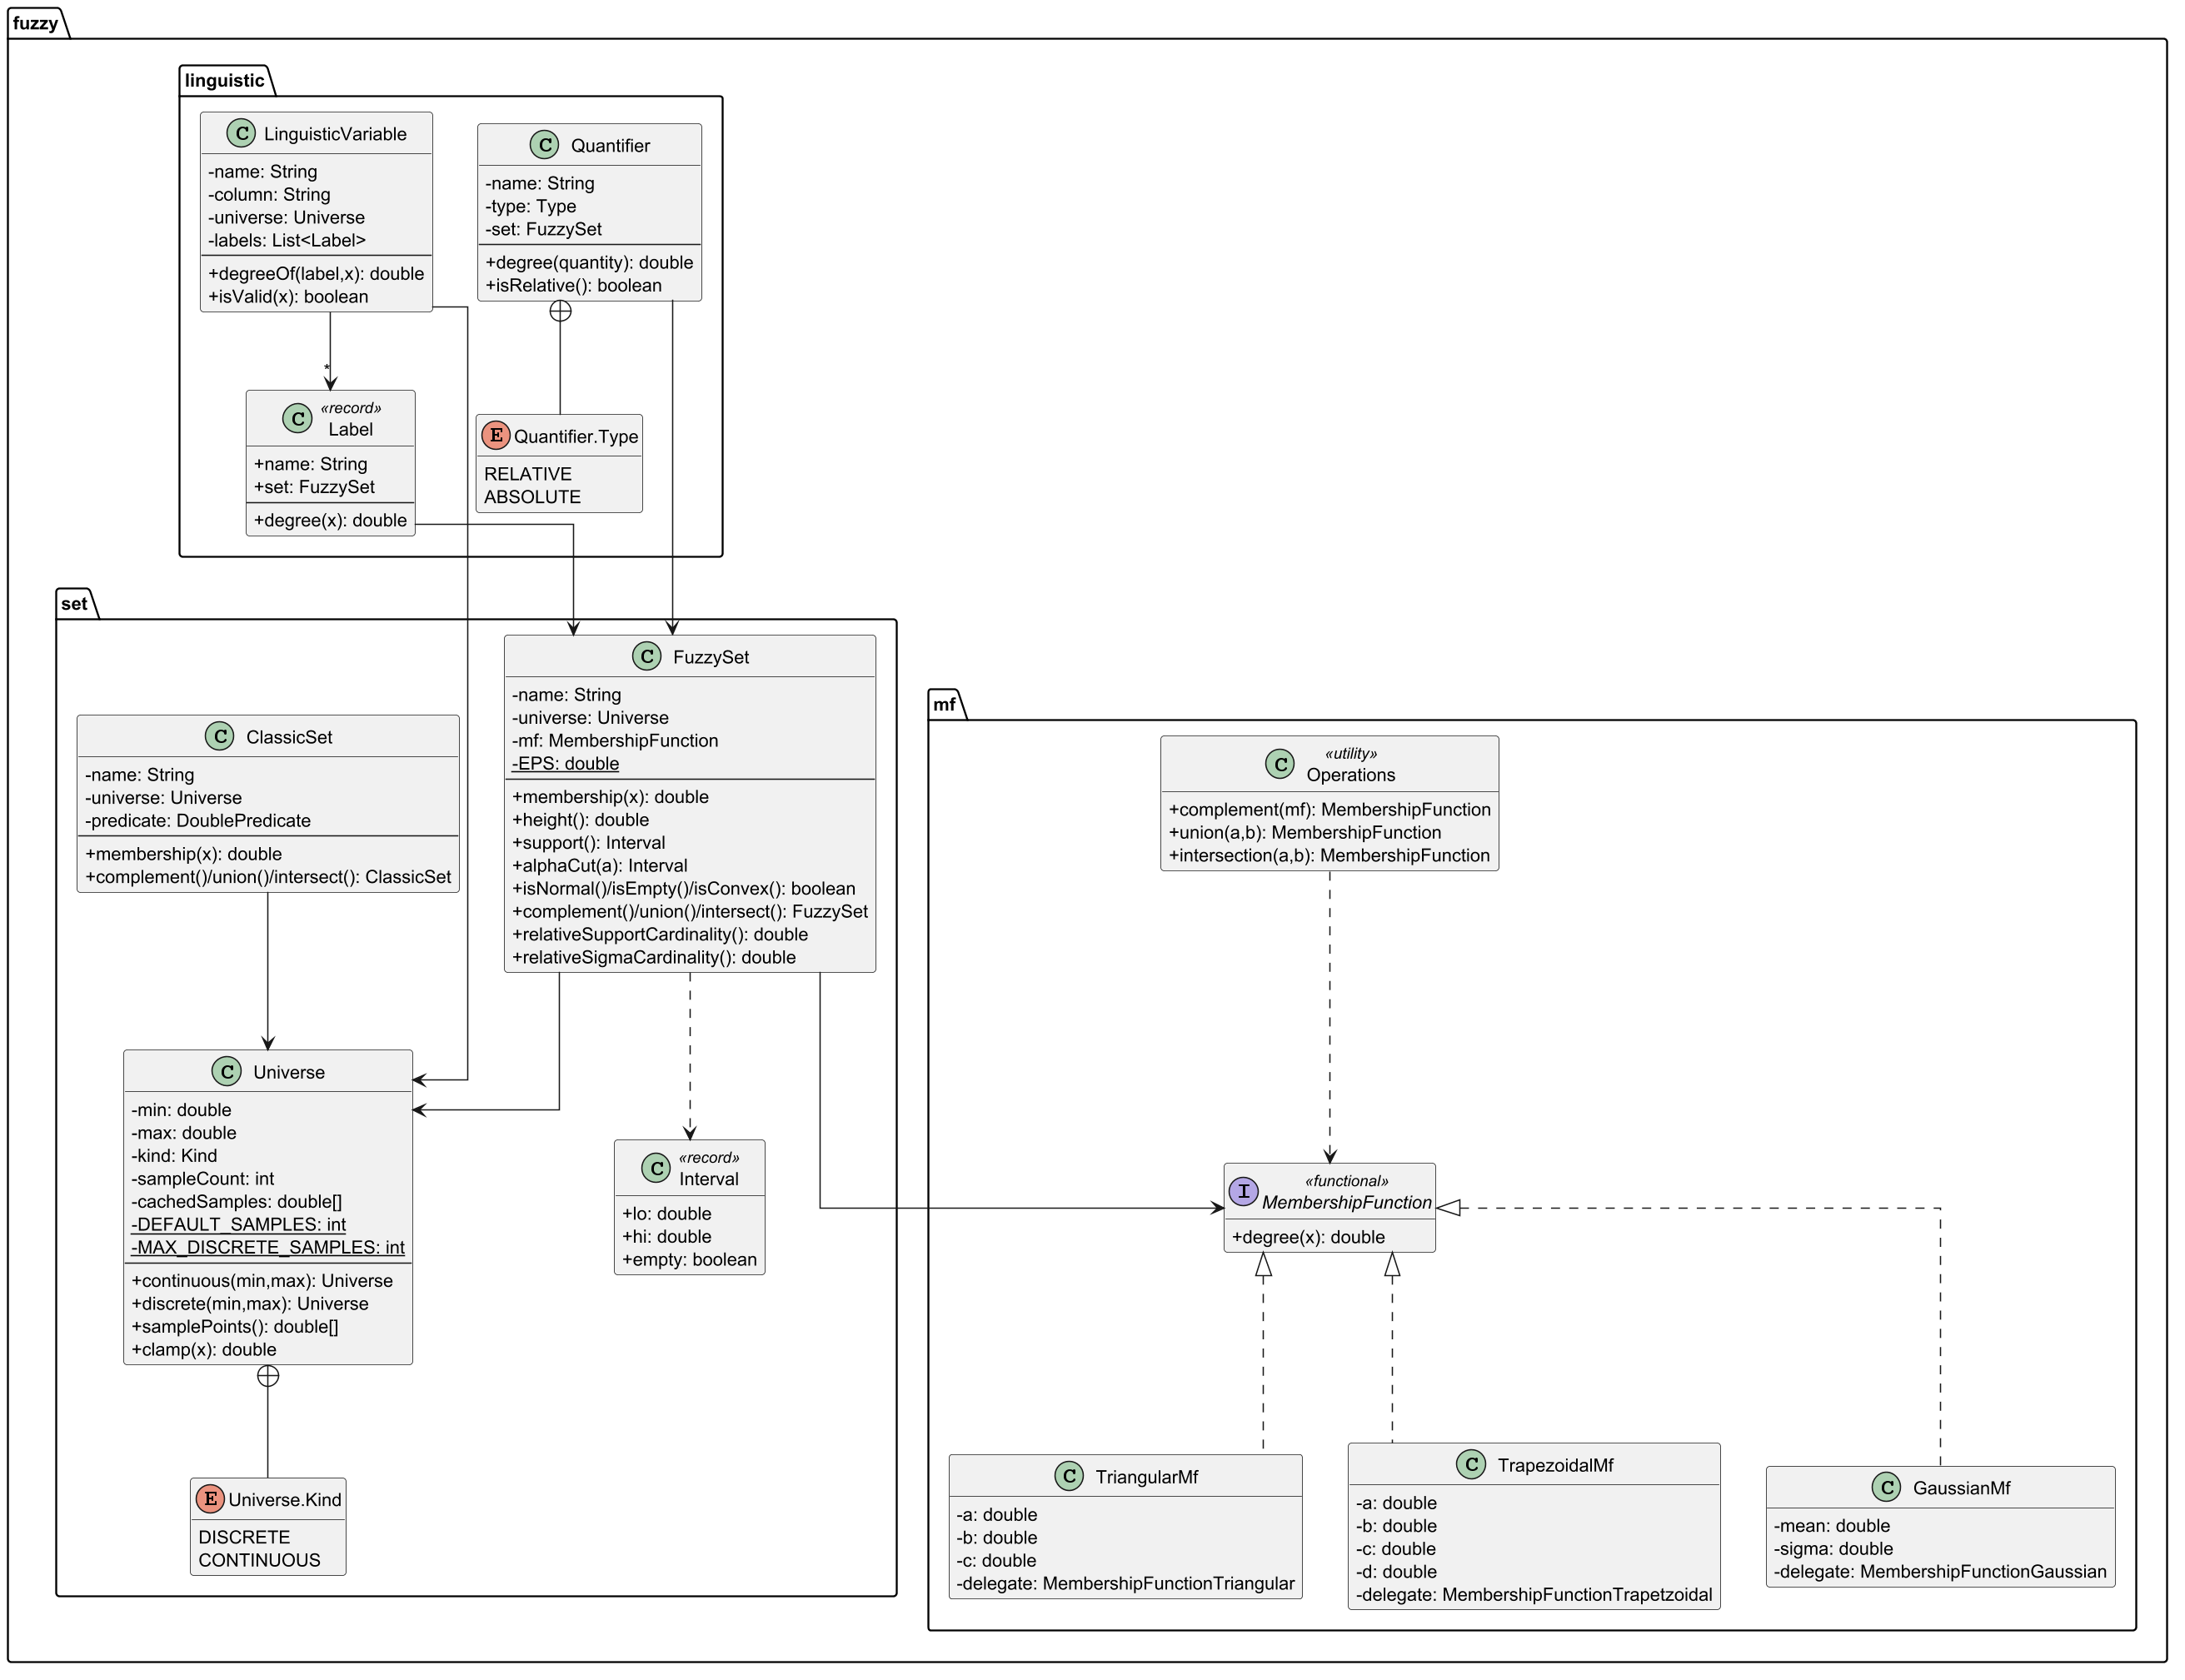
\includegraphics[width=0.88\linewidth]{uml_fuzzy.png}
    \caption{Warstwa zbiorów rozmytych, uniwersów i funkcji przynależności.}
\end{figure}

\subsection{Warstwa konfiguracji}

\code{FuzzyConfig} jest centralnym miejscem konfiguracji. Tworzy:

\begin{itemize}
    \item listę zmiennych lingwistycznych;
    \item listę kwantyfikatorów względnych;
    \item listę kwantyfikatorów absolutnych;
    \item metody pomocnicze do dodawania własnych etykiet i kwantyfikatorów.
\end{itemize}

Jeżeli chcesz zmienić znaczenie słowa \emph{duża moc}, to właśnie tutaj szukasz parametrów funkcji przynależności. Jeżeli chcesz dodać nowy kwantyfikator typu \emph{około jedna trzecia}, też zaczynasz od tej warstwy.

\subsection{Warstwa generowania zdań}

\code{SummaryGenerator} działa na zasadzie kombinatorycznej:

\begin{itemize}
    \item bierze kwantyfikatory;
    \item bierze właściwości zbudowane z etykiet;
    \item składa je w zdania formy I albo II;
    \item dla złożonych sumaryzatorów używa \code{AND}/\code{OR}.
\end{itemize}

Sama składnia zdania jest osobną sprawą. Projekt ma pomocniczą klasę \code{SentenceGrammar}, która poprawia brzmienie generowanych zdań po polsku, np. dobiera frazy tak, żeby nie brzmiały jak mechanicznie sklejone fragmenty.

\subsection{Warstwa oceny jakości}

\code{QualityMeasures.evaluate} przechodzi po rekordach i zbiera wartości potrzebne do T1--T11:

\begin{itemize}
    \item stopnie sumaryzatora;
    \item stopnie kwalifikatora;
    \item liczby rekordów z dodatnią przynależnością;
    \item rozmyte liczności;
    \item nośniki i kardynalności etykiet.
\end{itemize}

Wynikiem jest obiekt \code{Quality}, który przechowuje wartości T1--T11 oraz \code{optimal}.

\subsection{Warstwa GUI}

\code{SummaryGui} jest aplikacją Swing. Ona nie implementuje teorii od zera, tylko łączy warstwy:

\begin{itemize}
    \item ładuje dane;
    \item pozwala użytkownikowi wybrać formę podsumowań;
    \item uruchamia generator;
    \item liczy miary;
    \item pokazuje tabelę;
    \item eksportuje CSV;
    \item pozwala dodawać nowe etykiety i kwantyfikatory w trybie zaawansowanym.
\end{itemize}

\begin{figure}[htbp]
    \centering
    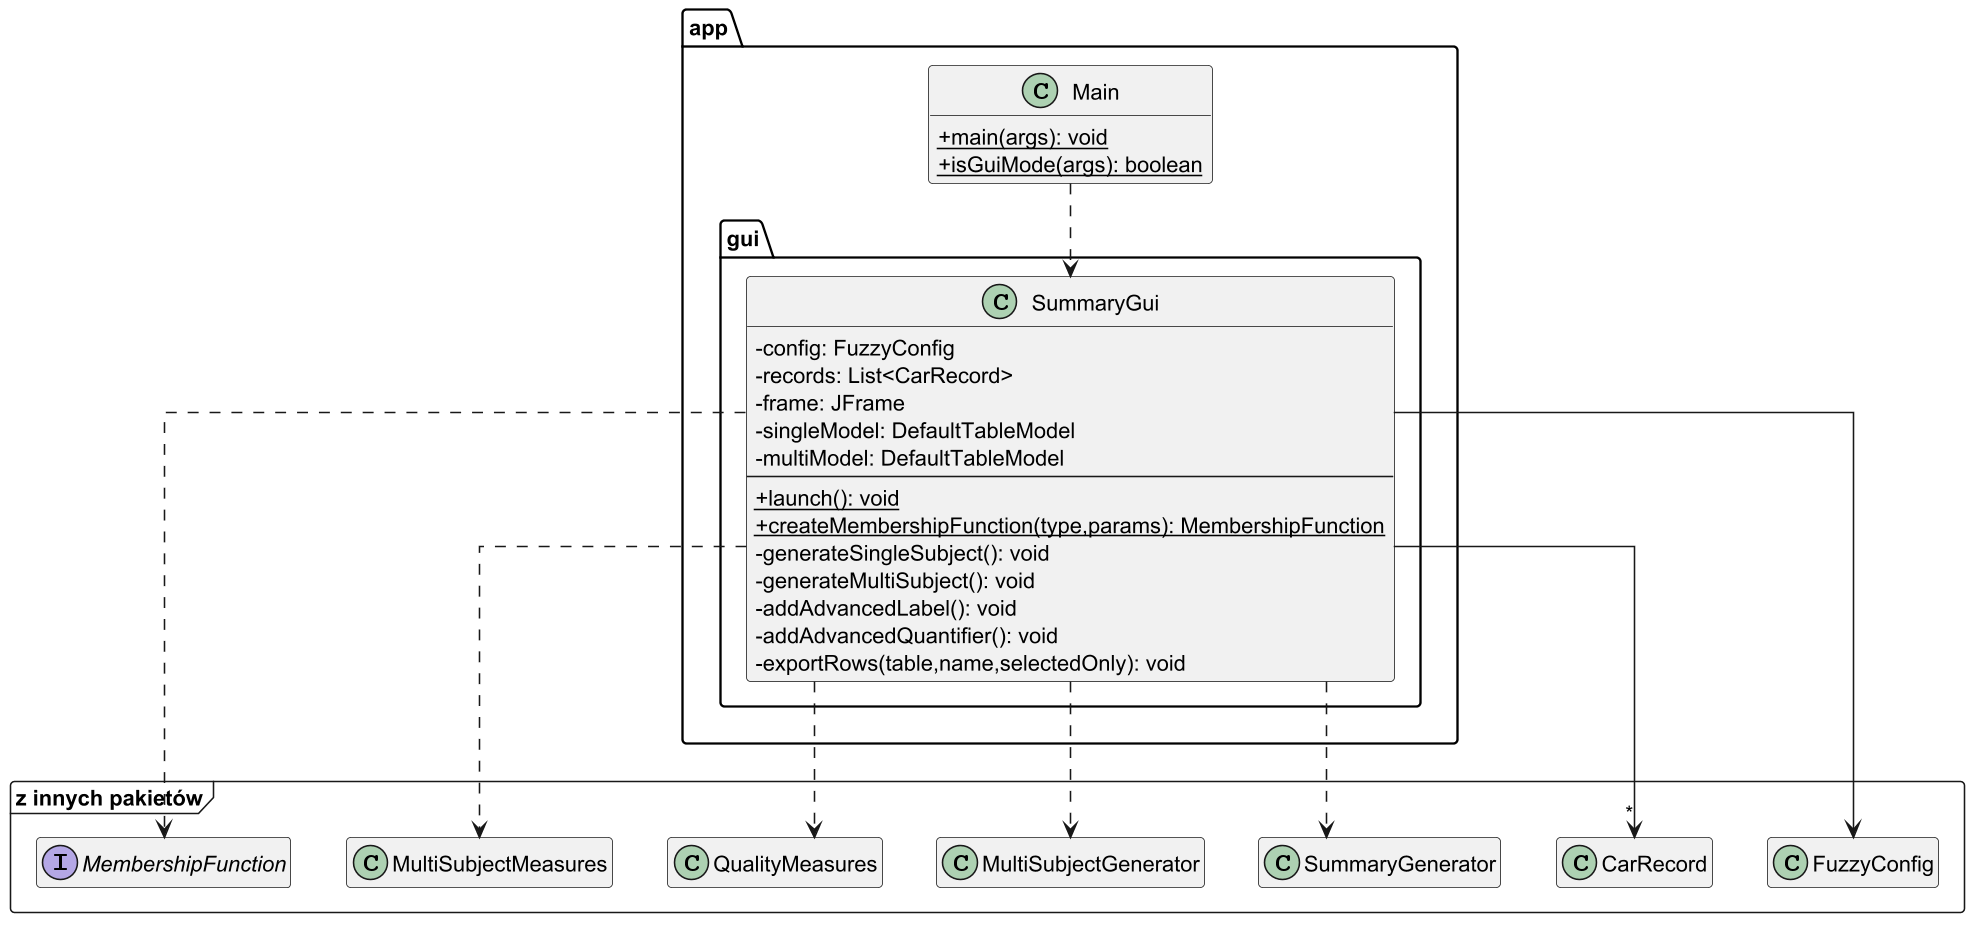
\includegraphics[width=0.92\linewidth]{uml_gui.png}
    \caption{GUI jako warstwa spinająca dane, konfigurację, generatory i wyniki.}
\end{figure}

\section{GUI: jak działa aplikacja}

\subsection{Uruchomienie}

Punkt startowy to \code{Main}. Aplikacja ładuje dane i uruchamia GUI. Jeżeli baza SQLite nie istnieje albo dane wymagają przygotowania, wykorzystywane są komponenty importu i czyszczenia.

Projekt jest Mavenowy, więc typowy workflow programistyczny to:

\begin{lstlisting}[style=javacode]
mvn test
mvn exec:java
\end{lstlisting}

Pierwsza komenda uruchamia testy, druga aplikację.

\subsection{Zakładka jednopodmiotowa}

W tej zakładce użytkownik tworzy podsumowania dla całej bazy samochodów. Może wybrać:

\begin{itemize}
    \item formę I albo II;
    \item kwantyfikatory względne albo absolutne;
    \item sumaryzator;
    \item kwalifikator dla formy II;
    \item spójnik dla podsumowań złożonych;
    \item miarę sortowania, np. \code{OPT} albo \code{T1};
    \item liczbę najlepszych wyników;
    \item wagi T1--T11.
\end{itemize}

Najważniejsza praktyczna decyzja: sortowanie po \code{T1} pokaże zdania najbardziej prawdziwe, a sortowanie po \code{OPT} pokaże zdania najlepsze według wybranego kompromisu wielu miar.

\subsection{Zakładka wielopodmiotowa}

Ta zakładka porównuje dwie grupy, najczęściej dwie marki. Użytkownik wybiera:

\begin{itemize}
    \item podmiot P1;
    \item podmiot P2;
    \item formę I--IV;
    \item sumaryzator;
    \item kwalifikator dla form II/III;
    \item kwantyfikator względny;
    \item sortowanie rosnące albo malejące po stopniu prawdziwości.
\end{itemize}

W podsumowaniach wielopodmiotowych kluczowa jest interpretacja argumentu kwantyfikatora. Nie chodzi tylko o to, czy P1 spełnia cechę, ale czy spełnia ją mocniej niż P2.

\subsection{Tryb zaawansowany}

Tryb zaawansowany pozwala rozszerzać system bez zmiany kodu:

\begin{itemize}
    \item dodać nową etykietę do zmiennej lingwistycznej;
    \item wybrać funkcję trójkątną, trapezoidalną albo gaussowską;
    \item podać parametry funkcji;
    \item dodać nowy kwantyfikator względny;
    \item dodać nowy kwantyfikator absolutny.
\end{itemize}

To jest ważne dydaktycznie, bo pozwala zobaczyć, że teoria nie jest zamknięta na sztywno. Granice pojęć językowych są modelowane przez parametry, a parametry można zmieniać i obserwować wpływ na wyniki.

\subsection{Eksport wyników}

GUI pozwala eksportować wyniki do CSV. To umożliwia dalszą analizę poza aplikacją, np. w arkuszu kalkulacyjnym. Eksport ma sens szczególnie wtedy, gdy chcemy porównać rankingi dla różnych wag albo różnych form zdań.

\section{Jak czytać wygenerowane wyniki}

\subsection{Nie patrz tylko na jedno pole}

Najczęstszy błąd to potraktowanie \code{OPT} jako jedynej prawdy. \code{OPT} jest kompromisem. Jeżeli wagi mocno premiują krótkość i precyzję, zdanie z niższym T1 może wyjść wysoko.

Rozsądna procedura interpretacji:

\begin{enumerate}
    \item Sprawdź tekst zdania.
    \item Sprawdź T1: czy zdanie jest rzeczywiście prawdziwe w danych?
    \item Sprawdź T3: czy dotyczy dużej części danych, czy niszy?
    \item Sprawdź T2 i T8: czy sumaryzator jest konkretny?
    \item Jeżeli jest kwalifikator, sprawdź T9--T11.
    \item Dopiero potem patrz na \code{OPT}.
\end{enumerate}

\subsection{Przykład interpretacyjny}

Zdanie:

\begin{center}
\emph{Większość samochodów ma małą pojemność silnika.}
\end{center}

Może mieć wysokie T1, jeżeli rozmyta średnia przynależność do etykiety \emph{mała pojemność} trafia w obszar kwantyfikatora \emph{większość}. Ale jeżeli etykieta \emph{mała pojemność} jest bardzo szeroka, T2 i T8 mogą być niższe. Wtedy zdanie jest prawdziwe, ale niekoniecznie bardzo precyzyjne.

Zdanie:

\begin{center}
\emph{Prawie żaden samochód ma bardzo dużą pojemność silnika.}
\end{center}

Może być prawdziwe, jeśli takich samochodów jest mało. Ale z punktu widzenia użytkownika warto jeszcze sprawdzić, czy etykieta \emph{bardzo duża pojemność} nie jest zdefiniowana zbyt wąsko. Jeżeli granice etykiety są bardzo ostre lub bardzo przesunięte, wynik może mówić bardziej o konfiguracji niż o danych.

\subsection{Interpretacja zdań z kwalifikatorem}

Zdanie:

\begin{center}
\emph{Większość samochodów o dużej mocy silnika ma dużą prędkość maksymalną.}
\end{center}

nie mówi o wszystkich samochodach. Mówi tylko o rozmytej grupie samochodów o dużej mocy. Jeśli kwalifikator obejmuje mało rekordów, T1 może być wysokie, ale T9/T10 powiedzą, że kwalifikator jest bardzo selektywny.

\subsection{Interpretacja wielopodmiotowa}

Zdanie:

\begin{center}
\emph{Większość samochodów marki BMW w porównaniu do samochodów marki Toyota ma dużą moc silnika.}
\end{center}

nie oznacza dosłownie, że większość wszystkich BMW ma dużą moc. Oznacza, że w porównaniu rozmytych udziałów między BMW i Toyotą cecha \emph{duża moc} wypada bardziej po stronie BMW zgodnie z kwantyfikatorem.

To jest bardzo ważne: w podsumowaniach wielopodmiotowych kwantyfikator opisuje relację między dwiema grupami, nie zwykły udział w jednej grupie.

\section{Najważniejsze klasy: przewodnik po kodzie}

\subsection{\code{CarRecord}}

\code{CarRecord} reprezentuje jeden rekord samochodu. To obiekt, z którego \code{Property} pobiera wartości kolumn. Jeżeli w danych wartość jest niepoprawna albo brakująca, dalsze warstwy muszą ją pominąć lub potraktować jako niemożliwą do oceny.

\subsection{\code{Columns}}

\code{Columns} centralizuje nazwy kolumn. Dzięki temu reszta kodu nie musi wpisywać nazw tekstowych w wielu miejscach. To ogranicza ryzyko literówek i ułatwia zmianę źródła danych.

\subsection{\code{DataCleaner}}

\code{DataCleaner} odpowiada za przygotowanie zbioru użytecznego w projekcie. To ważne, bo podsumowania lingwistyczne są wrażliwe na śmieci w danych. Niepoprawne lub brakujące wartości mogłyby zniekształcić stopnie przynależności.

\subsection{\code{FuzzyConfig}}

\code{FuzzyConfig} jest mapą semantyczną projektu. To tutaj surowe kolumny stają się pojęciami językowymi.

Przykład zależności:

\[
\code{engine\_hp} \rightarrow \text{moc silnika} \rightarrow
\{\text{bardzo mała}, \text{mała}, \text{średnia}, \text{duża}, \text{bardzo duża}\}
\]

Jeżeli ktoś pyta, gdzie w projekcie zdefiniowano znaczenie słów, odpowiedź brzmi: głównie w \code{FuzzyConfig}.

\subsection{\code{Property}}

\code{Property} to atom logiczno-lingwistyczny: zmienna plus etykieta. Na przykład:

\[
\text{moc silnika} + \text{duża}
\]

Dla rekordu samochodu \code{Property} zwraca stopień, np. 0.73. Generator i miary jakości nie muszą znać szczegółów kolumn ani funkcji przynależności, bo \code{Property} ukrywa ten mechanizm.

\subsection{\code{LabelExpression}}

\code{LabelExpression} reprezentuje wyrażenie złożone z etykiet. Dzięki temu sumaryzator albo kwalifikator może być traktowany jednolicie niezależnie od tego, czy jest pojedynczy, czy złożony.

\subsection{\code{SummaryGenerator}}

\code{SummaryGenerator} tworzy kandydatów podsumowań. To generator zdań, a nie oceniacz. Jego zadaniem jest poprawnie złożyć kwantyfikator, sumaryzator, ewentualny kwalifikator i tekst.

\subsection{\code{QualityMeasures}}

\code{QualityMeasures} jest matematycznym centrum oceny. Dla każdego podsumowania przechodzi po rekordach i liczy:

\begin{itemize}
    \item stopień prawdziwości;
    \item pokrycie;
    \item precyzję;
    \item długość;
    \item miary kwantyfikatora;
    \item miary kwalifikatora;
    \item wynik optymalny.
\end{itemize}

Jeżeli trzeba debugować ,,dlaczego to zdanie ma taki wynik'', najczęściej kończy się właśnie tutaj.

\subsection{\code{MultiSubjectGenerator} i \code{MultiSubjectMeasures}}

Te klasy robią analogiczne rzeczy dla zdań porównujących dwa podmioty:

\begin{itemize}
    \item generator tworzy zdania form I--IV;
    \item miary liczą stopień prawdziwości porównania.
\end{itemize}

Projekt nie liczy pełnego zestawu T1--T11 dla wielopodmiotowych zdań, tylko stopień prawdziwości. To jest zgodne z zakresem implementacji: wielopodmiotowa część skupia się na porównaniu, a nie na pełnym rankingu jakości znanym z jednopodmiotowych podsumowań.

\subsection{\code{SummaryGui}}

\code{SummaryGui} jest największą klasą interfejsu. Warto czytać ją nie jako teorię, tylko jako orkiestrację:

\begin{itemize}
    \item tworzy komponenty Swing;
    \item reaguje na kliknięcia;
    \item wywołuje generatory;
    \item pokazuje tabele;
    \item obsługuje eksport;
    \item dodaje konfiguracje z trybu zaawansowanego.
\end{itemize}

\section{Od zdania do wyniku: pełny przykład}

Weźmy zdanie:

\begin{center}
\emph{Większość samochodów ma małą pojemność silnika.}
\end{center}

\subsection{Krok 1: wybór kwantyfikatora}

Kwantyfikator:

\[
Q=\text{większość}
\]

Jest względny, więc jego dziedziną jest \([0,1]\).

\subsection{Krok 2: wybór sumaryzatora}

Sumaryzator:

\[
S=\text{mała pojemność silnika}
\]

To \code{Property} złożone ze zmiennej \emph{pojemność silnika} i etykiety \emph{mała}.

\subsection{Krok 3: ocena każdego rekordu}

Dla każdego samochodu:

\begin{enumerate}
    \item pobieramy \code{capacity\_cm3};
    \item liczymy \(\mu_S(capacity)\);
    \item dodajemy wynik do sumy.
\end{enumerate}

Przykładowo:

\[
1000 \mapsto 1.0,\quad 1600 \mapsto 0.7,\quad 2200 \mapsto 0.1,\quad 4000 \mapsto 0.0
\]

\subsection{Krok 4: agregacja}

Jeżeli mamy \(n\) rekordów:

\[
r=\frac{1}{n}\sum_{i=1}^{n}\mu_S(y_i)
\]

To jest rozmyty udział samochodów o małej pojemności.

\subsection{Krok 5: zastosowanie kwantyfikatora}

Stopień prawdziwości:

\[
T_1=\mu_{\text{większość}}(r)
\]

Jeżeli \(r=0.75\), a kwantyfikator \emph{większość} ma plateau w okolicach 0.70--0.85, T1 może wynieść 1.0.

\subsection{Krok 6: pozostałe miary}

Następnie liczymy T2--T11:

\begin{itemize}
    \item T2/T8 z kształtu etykiety \emph{mała pojemność};
    \item T3 z liczby rekordów o dodatniej przynależności;
    \item T5 z długości sumaryzatora;
    \item T6/T7 z kwantyfikatora \emph{większość};
    \item T9--T11 są 0, bo nie ma kwalifikatora.
\end{itemize}

\section{Co zmienia konfiguracja funkcji przynależności}

\subsection{Granice słów są decyzją projektową}

To, czy samochód o mocy 150 KM jest \emph{mocny}, zależy od parametrów etykiety. W tym sensie podsumowania lingwistyczne nie są czystą statystyką. Są statystyką przepuszczoną przez model znaczeń językowych.

Jeżeli przesuniemy etykietę \emph{duża moc} w prawo, mniej samochodów będzie do niej należeć. Zmieni się:

\begin{itemize}
    \item T1 dla zdań z tą etykietą;
    \item T3, bo mniej rekordów będzie miało dodatnie pokrycie;
    \item T2 i T8, bo zmieni się kształt/nośnik/kardynalność etykiety;
    \item rankingi w GUI.
\end{itemize}

\subsection{Dlaczego wykresy są ważne}

Wykresy funkcji przynależności pozwalają zobaczyć, co naprawdę znaczą słowa. Bez wykresu łatwo założyć, że \emph{duży} znaczy to samo dla każdego. W systemie znaczy dokładnie tyle, ile opisują parametry funkcji.

\begin{figure}[htbp]
    \centering
    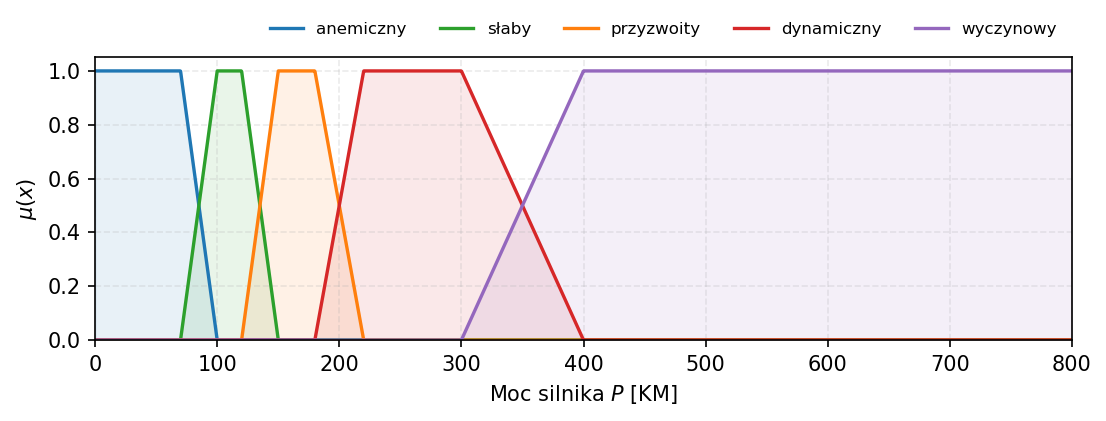
\includegraphics[width=0.82\linewidth]{mf_engine_hp.png}
    \caption{Etykiety dla mocy silnika.}
\end{figure}

\begin{figure}[htbp]
    \centering
    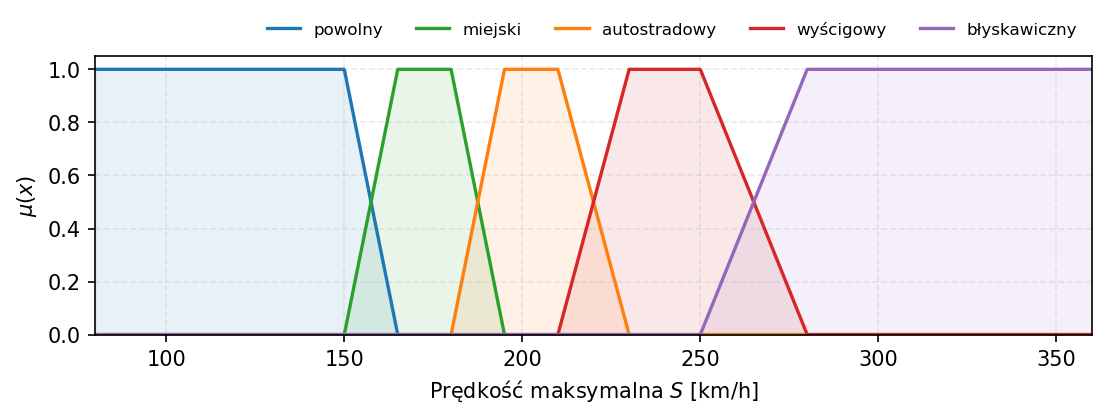
\includegraphics[width=0.82\linewidth]{mf_max_speed_km_per_h.png}
    \caption{Etykiety dla prędkości maksymalnej.}
\end{figure}

\section{Testy i poprawność}

\subsection{Co sprawdzają testy}

Testy w projekcie obejmują między innymi:

\begin{itemize}
    \item uruchamialność głównej aplikacji;
    \item działanie konfiguracji zaawansowanej;
    \item komponenty GUI w zakresie możliwym do automatycznego sprawdzenia;
    \item miary podsumowań wielopodmiotowych.
\end{itemize}

Testy nie zastępują interpretacji matematycznej, ale chronią przed regresjami: jeżeli zmiana w generatorze albo miarach psuje oczekiwane zachowanie, Maven powinien to wykryć.

\subsection{Co trzeba sprawdzać ręcznie}

Nie wszystko da się łatwo sprawdzić testem jednostkowym:

\begin{itemize}
    \item naturalność językowa zdań po polsku;
    \item sens dobranych granic etykiet;
    \item interpretacyjna przydatność rankingów;
    \item czy GUI jest ergonomiczne dla użytkownika;
    \item czy wykresy i UML-e w sprawozdaniu odpowiadają aktualnemu kodowi.
\end{itemize}

Dlatego pełna ocena projektu wymaga zarówno testów, jak i czytania sprawozdania, kodu oraz wyników działania aplikacji.

\section{Najczęstsze pułapki}

\subsection{Pomylenie kwantyfikatora względnego z absolutnym}

\emph{Większość} działa na proporcji. \emph{Kilka tysięcy} działa na liczbie. Jeżeli podstawimy zły typ argumentu, wynik nie ma sensu.

\subsection{Traktowanie stopnia przynależności jak prawdopodobieństwa}

\(\mu_A(x)=0.7\) nie znaczy, że prawdopodobieństwo przynależności wynosi 70\%. Znaczy, że wartość pasuje do pojęcia \(A\) w stopniu 0.7. To jest semantyczna zgodność z pojęciem, nie losowość.

\subsection{Traktowanie T1 jako jedynej miary jakości}

T1 mówi o prawdziwości. Nie mówi pełnej historii o precyzji, długości, selektywności ani informacyjności. Dlatego w tabelach są T1--T11.

\subsection{Zapominanie o kwalifikatorze}

Zdanie z kwalifikatorem mówi o podzbiorze rozmytym. Jeśli kwalifikator jest bardzo wąski, zdanie może być prawdziwe, ale dotyczyć niewielkiej części danych.

\subsection{Mylenie form wielopodmiotowych}

Forma I, II, III i IV nie są kosmetycznymi wariantami tekstu. Różnią się tym, jak liczą porównanie i gdzie stosują kwalifikator.

\section{Ściąga pojęć}

\begin{longtable}{p{0.25\linewidth}p{0.65\linewidth}}
\toprule
\textbf{Pojęcie} & \textbf{Znaczenie}\\
\midrule
\endhead
uniwersum & dziedzina wartości, np. zakres mocy silnika\\
zbiór rozmyty & zbiór opisany funkcją przynależności do \([0,1]\)\\
funkcja przynależności & zamienia wartość liczbową na stopień pasowania do pojęcia\\
etykieta & nazwa językowa plus zbiór rozmyty, np. \emph{duża moc}\\
zmienna lingwistyczna & atrybut opisany etykietami, np. \emph{moc silnika}\\
kwantyfikator & rozmyte określenie liczności lub proporcji, np. \emph{większość}\\
kwantyfikator względny & działa na proporcji \([0,1]\)\\
kwantyfikator absolutny & działa na liczności\\
sumaryzator & cecha przypisywana obiektom w zdaniu\\
kwalifikator & cecha zawężająca zbiór obiektów\\
podmiot & zbiór obiektów, np. wszystkie samochody albo marka BMW\\
T1 & stopień prawdziwości zdania\\
OPT & średnia ważona T1--T11\\
\bottomrule
\end{longtable}

\section{Ściąga po klasach}

\begin{longtable}{p{0.30\linewidth}p{0.60\linewidth}}
\toprule
\textbf{Klasa} & \textbf{Rola}\\
\midrule
\endhead
\code{Main} & uruchamia aplikację\\
\code{SummaryGui} & interfejs użytkownika\\
\code{CarRecord} & jeden rekord samochodu\\
\code{CarDataLoader} & ładuje rekordy z bazy/danych\\
\code{DataCleaner} & przygotowuje oczyszczony zbiór danych\\
\code{Universe} & dziedzina dla zbioru rozmytego\\
\code{FuzzySet} & zbiór rozmyty i operacje na nim\\
\code{ClassicSet} & klasyczny predykat zbioru\\
\code{MembershipFunction} & interfejs funkcji przynależności\\
\code{TriangularMf} & funkcja trójkątna\\
\code{TrapezoidalMf} & funkcja trapezoidalna\\
\code{GaussianMf} & funkcja gaussowska\\
\code{Label} & etykieta lingwistyczna\\
\code{LinguisticVariable} & zmienna lingwistyczna\\
\code{Quantifier} & kwantyfikator względny lub absolutny\\
\code{Property} & atom sumaryzatora/kwalifikatora\\
\code{Connective} & spójniki AND/OR\\
\code{SummaryGenerator} & generator podsumowań jednopodmiotowych\\
\code{SingleSubjectSummary} & obiekt zdania jednopodmiotowego\\
\code{QualityMeasures} & obliczanie T1--T11\\
\code{QualityWeights} & wagi do wyniku optymalnego\\
\code{Subject} & podmiot w porównaniu wielopodmiotowym\\
\code{MultiSubjectGenerator} & generator zdań wielopodmiotowych\\
\code{MultiSubjectMeasures} & prawdziwość zdań wielopodmiotowych\\
\bottomrule
\end{longtable}

\section{Jak wytłumaczyć projekt komuś na głos}

Jeżeli masz opowiedzieć ten projekt na zajęciach albo obronić jego sens, dobry schemat wypowiedzi jest taki:

\begin{enumerate}
    \item Mamy bazę samochodów i chcemy generować z niej zdania opisowe, a nie tylko statystyki.
    \item Ponieważ pojęcia typu \emph{duży}, \emph{mały}, \emph{szybki} są nieostre, używamy logiki rozmytej.
    \item Każda zmienna liczbowa ma etykiety lingwistyczne opisane funkcjami przynależności.
    \item Kwantyfikatory, takie jak \emph{większość}, też są zbiorami rozmytymi.
    \item Generator składa zdania z kwantyfikatora, podmiotu, sumaryzatora i opcjonalnego kwalifikatora.
    \item Miara T1 mówi, na ile zdanie jest prawdziwe w danych.
    \item Miary T2--T11 oceniają dodatkowo precyzję, pokrycie, długość, kwantyfikator i kwalifikator.
    \item GUI pozwala wybierać formy zdań, sortować wyniki, zmieniać wagi i dodawać własne etykiety.
    \item Wersja wielopodmiotowa porównuje dwie grupy, np. marki samochodów.
    \item Całość jest zaimplementowana warstwowo: dane, logika rozmyta, konfiguracja lingwistyczna, generatory, miary, GUI.
\end{enumerate}

\section{Bibliografia orientacyjna}

Ten dokument korzysta z teorii i materiałów opisanych w sprawozdaniu projektu, w szczególności z klasycznego podejścia do podsumowań lingwistycznych baz danych i logiki rozmytej:

\begin{itemize}
    \item L. A. Zadeh, prace o zbiorach rozmytych, zmiennych lingwistycznych i kwantyfikatorach rozmytych.
    \item R. R. Yager, koncepcja lingwistycznych podsumowań danych.
    \item J. Kacprzyk, R. R. Yager, S. Zadrożny, prace o podsumowaniach lingwistycznych baz danych.
    \item A. Niewiadomski, materiały wykładowe i publikacje dotyczące podsumowań lingwistycznych.
    \item Dokumentacja i kod projektu \code{linguistic-summaries}.
\end{itemize}

\section*{Zakończenie}
\addcontentsline{toc}{section}{Zakończenie}

Cały projekt można streścić jednym zdaniem: jest to system, który modeluje nieostre pojęcia językowe matematycznie, stosuje je do rekordów samochodów, generuje zdania opisujące dane i ocenia te zdania wieloma miarami jakości.

Najważniejsze jest zrozumienie mostu między językiem a matematyką:

\[
\begin{aligned}
\text{słowo} &\rightarrow \text{etykieta} \rightarrow \text{funkcja przynależności}\\
&\rightarrow \text{stopnie dla rekordów} \rightarrow \text{podsumowanie} \rightarrow \text{miary jakości}
\end{aligned}
\]

Gdy ten łańcuch jest jasny, reszta kodu staje się dużo mniej tajemnicza: klasy nie są przypadkowymi elementami aplikacji, tylko kolejnymi poziomami tej samej idei.

\end{document}
